% ŠABLONA PRO PSANÍ SOČ
%%%%%%%%%%%%%%%%%%%%%%%%%
% Autor: Jakub Dokulil (kubadokulil99@gmail.com)
% Tato šablona byla vytvořena tak, aby pomocí ní mohli v systému LaTeX soutěžící sázet své práce a zároveň odpovídala požadavkům na formátování vyplývajícím z wordové šablony umístěné na webu soc.cz.
%

% !TEX root = ./main.tex

\documentclass[12pt, a4paper,
  %oneside,      %% -- odkomentujte, pokud chcete svou práci mít pouze jednostrannou, mezera pro hřbet pak automaticky bude pouze na levé straně
 twoside,        %% -- pro oboustranné práce, mezera pro hřbet následně střídá strany.
 openright
]{report}

%% Nutné balíčky a nastavení
%%%%%%%%%%%%%%%%%%%%%%%%%%%%

%% Proměnné
\newcommand\city{Praha} %% vyplň oficiální název města
\newcommand\district{Hlavní město Praha} %% vyplň oficiální název kraje
\newcommand\specialization{Obor č. 2: Fyzika} %% -- napiš číslo a název tvého oboru
\newcommand\school{Gymnázium Christiana Dopplera} %% vyplň název školy
\newcommand\schoolAddress{Zborovská 621, 150 00 Malá Strana} %% vyplň název školy
\newcommand\consultant{RNDr. Pavel Josef, CSc.} %% vyplň jméno svého konzultanta
\newcommand\authorName{Ondřej Sedláček}  %% vyplň své jméno
\newcommand\publicationYear{2023} %% vyplň rok
\newcommand\mainTitle{Počítačové modelování dynamických magnetických systémů} %% vyplň název své práce
\newcommand\mainTitleEN{Computer modelling of dynamic magnetic systems} %% vyplň název své práce

\title{\mainTitle} %% -- Název tvé práce
\author{\authorName} %% -- tvé jméno
\date{\publicationYear} %% -- rok, kdy píšeš SOČku

\usepackage[top=2.5cm, bottom=2.5cm, left=3.5cm, right=1.5cm]{geometry} %% nastaví okraje, left -- vnitřní okraj, right -- vnější okraj

\usepackage[english, czech]{babel} %% balík babel pro sazbu v češtině
\usepackage[utf8]{inputenc} %% balíky pro kódování textu
\usepackage[T1]{fontenc}
\usepackage{cmap} %% balíček zajišťující, že vytvořené PDF bude prohledávatelné a kopírovatelné

\usepackage{graphicx} %% balík pro vkládání obrázků
\usepackage{mathtools}
\usepackage{subcaption} %% balíček pro vkládání podobrázků
\usepackage{wrapfig}
\usepackage{setspace}

\linespread{1.15} %% řádkování

\usepackage[pagestyles]{titlesec} %% balíček pro úpravu stylu kapitol a sekcí
\titleformat{\chapter}[block]{\scshape\bfseries\LARGE}{\thechapter}{10pt}{\vspace{0pt}}[\vspace{-22pt}]
\titleformat{\section}[block]{\scshape\bfseries\Large}{\thesection}{10pt}{\vspace{0pt}}
\titleformat{\subsection}[block]{\bfseries\large}{\thesubsection}{10pt}{\vspace{0pt}}

\setcounter{secnumdepth}{2}
\setcounter{tocdepth}{4}
\usepackage{fancyhdr}
\usepackage{listings}
\usepackage{chngcntr}

\pagestyle{fancy}
\renewcommand{\headrulewidth}{1pt}

\usepackage{xcolor}

\definecolor{codegreen}{rgb}{0,0.6,0}
\definecolor{codegray}{rgb}{0.5,0.5,0.5}
\definecolor{codepurple}{rgb}{0.58,0,0.82}
\definecolor{backcolour}{rgb}{0.95,0.95,0.92}

\lstdefinestyle{mystyle}{
    backgroundcolor=\color{backcolour},
    commentstyle=\color{codegreen},
    keywordstyle=\color{magenta},
    numberstyle=\tiny\color{codegray},
    stringstyle=\color{codepurple},
    basicstyle=\ttfamily\footnotesize,
    breakatwhitespace=false,
    breaklines=true,
    captionpos=b,
    keepspaces=true,
    numbers=left,
    numbersep=5pt,
    showspaces=false,
    showstringspaces=false,
    showtabs=false,
    tabsize=2
}

\addto\captionsczech{\renewcommand{\figurename}{Obr.}}
\addto\captionsczech{\renewcommand{\tablename}{Tab.}}
\counterwithout{figure}{chapter}
\counterwithout{table}{chapter}
\counterwithout{equation}{chapter}
\counterwithout{footnote}{chapter}

\lstset{style=mystyle}
\lstset{numberbychapter=false}
\renewcommand{\lstlistingname}{Ústřižek kódu}
\renewcommand{\lstlistlistingname}{Seznam ústřižků}

\setlength{\parskip}{12pt}%
\setlength{\parindent}{0pt}%

% \usepackage[]{nomencl}
% % makeindex main.nlo -s nomencl.ist -o main.nls
\usepackage{tabularx} % in the preamble
\usepackage{float}
\usepackage{booktabs}
\usepackage{url}

\usepackage{tikz}
\usetikzlibrary{shapes.geometric, arrows}

%% Balíčky co se můžou hodit :)
%%%%%%%%%%%%%%%%%%%%%%%%%%%%%%%

\usepackage{pdfpages} %% Balíček umožňující vkládat stránky z PDF souborů,

\usepackage{upgreek} %% Balíček pro sazbu stojatých řeckých písmen, třeba u jednotky mikrometr. Například stojaté mí: \upmu, stojaté pí: \uppi

\usepackage{amsmath}    %% Balíčky amsmath a amsfonts
\usepackage{amssymb}    %% Balíčky amsmath a amsfonts
\usepackage{yhmath}    %% Balíčky amsmath a amsfonts
\usepackage{amsfonts}   %% pro sazbu matematických symbolů
\usepackage{esint}     %% pro sazbu různých integrálů (např \oiint)
\usepackage{mathrsfs}
\usepackage{enumitem}

%% makra pro sazbu matematiky
\newcommand{\dif}{\mathrm{d}} %% makro pro sazbu diferenciálu, místo toho
%% abych musel psát '\mathrm{d}' mi stačí napsat '\dif' což je mnohem
%% kratší a mohu si tak usnadnit práci

%% Bordel pro práci - můžeš smáznout :)
%%%%%%%%%%%%%%%%%%%

\usepackage{lipsum} %% balíček který píše lipsum (nesmyslný text, který se používá pro kontrolu typografie)
\usepackage{tablefootnote}
\usepackage{dblfnote}
\DFNtrysingle
\DFNinhibitcbreak
\DFNcolumnwidth 1.1\textwidth
% \DFNsloppiness 1000

\makeatletter
\newcommand{\vast}{\bBigg@{3}}
\newcommand{\vastt}{\bBigg@{4}}
\newcommand{\Vast}{\bBigg@{5}}
\newcommand{\Vastt}{\bBigg@{6}}
\makeatother

\usepackage{tikz}
% %%%<
%     \PreviewEnvironment{tikzpicture}
%     \setlength\PreviewBorder{10pt}%
% %%%>
\usetikzlibrary{shapes.geometric}
\usetikzlibrary{shapes.arrows}
\usetikzlibrary{shapes.geometric, arrows,positioning}
\usetikzlibrary{calc}

\usepackage{hyperref} %% balíček, který v PDF vytváří odkazy
\renewcommand*{\figureautorefname}{Obr.}
\renewcommand*{\tableautorefname}{Tab.}
\renewcommand*{\equationautorefname}{Rov.}
\renewcommand*{\chapterautorefname}{Kap.}
\renewcommand*{\sectionautorefname}{Kap.}
\renewcommand*{\subsectionautorefname}{Kap.}
% \renewcommand*{\subsubsectionautorefname}{Kap.}

%% Začátek dokumentu
%%%%%%%%%%%%%%%%%%%%

\begin{document}
\pagestyle{empty}
\pagenumbering{Roman}
\graphicspath{{./imgsLR}}

% PŘEDNÍ STRANA
\begin{titlepage}
    \bfseries{ %%% písmo na stránce je tučně
        \begin{center}
            \LARGE{STŘEDOŠKOLSKÁ ODBORNÁ ČINNOST}

            \vspace{14pt}
            \large{ %%%%
                \specialization
            } %%%%

            \vspace{0.3 \textheight}

            \LARGE{ %%%%
                \mainTitle
            }%%%%

            \vspace{0.35 \textheight}
        \end{center}

        \noindent\Large{\authorName}

        \noindent\Large{\district \hspace{\stretch{1}}  \city, \publicationYear}


    } %%%
\end{titlepage}
\cleardoublepage

% ÚVODNÍ STRANA
% \begin{}
%% Úvodní stránka s informacemi
{\bfseries %%% písmo na stránce je tučně
    \begin{center}
        \LARGE{STŘEDOŠKOLSKÁ ODBORNÁ ČINNOST}

        \vspace{14pt}
        {\large %%%%
            \specialization %% -- napiš číslo a název tvého oboru
        } %%%%

        \vspace{0.20 \textheight}

        \LARGE{ %%%%
            \mainTitle
        }

        \LARGE{ %%%%
            \mainTitleEN
        }%%%%

        \vspace{0.25\textheight}
    \end{center}
}%%%
{\Large %%%
    \noindent\textbf{Jméno:} \authorName\\
    \textbf{Škola:} \school, \schoolAddress\\
    \textbf{Kraj:} \district\\
    \textbf{Konzultant:} \consultant\\
} %%%

\noindent \city, \publicationYear
% \end{}
\cleardoublepage

% PROHLÁŠENÍ
% \begin{}
\noindent{\Large{\bfseries{Prohlášení}}}

\noindent Prohlašuji, že jsem svou práci SOČ vypracoval samostatně a použil jsem pouze prameny a literaturu uvedené v seznamu bibliografických záznamů.

\noindent Prohlašuji, že tištěná verze a elektronická verze soutěžní práce SOČ jsou shodné.

\noindent Nemám závažný důvod proti zpřístupňování této práce v souladu se zákonem č. 121/2000 Sb., o právu autorském, o právech souvisejících s právem autorským a o změně některých zákonů (autorský zákon) ve znění pozdějších předpisů.

\vspace{24 pt}

\noindent V Praze dne 9. září 2023 \dotfill{}\hspace{\stretch{0.9}}

\hspace{6cm} \authorName
% \end{}
\cleardoublepage

% PODĚKOVÁNÍ TODO
% \begin{}
\vspace*{0.0\textheight}
% \vspace*{0.8\textheight}
\noindent{\Large{\bfseries{Poděkování}}}

\noindent
Chtěl bych poděkovat ...
% \end{}
\cleardoublepage

% ANOTACE TODO
% \begin{}
\noindent{\Large{\bfseries{Anotace}}}

\noindent Sem napíšeš svůj abstrakt. \lipsum[1] %% přepiš!!

\vspace{18pt}

% TODO - keywords
\noindent{\Large{\bfseries{Klíčová slova}}}

\noindent Šablona, \LaTeX, SOČ, \dots

\vspace{18pt}

% TODO - abstrakt EN
\noindent{\Large{\bfseries{Annotation}}}

\noindent Write your abstract here! \lipsum[1] %% přepiš!!

\vspace{18pt}

% TODO - keywords EN
\noindent{\Large{\bfseries{Keywords}}}

\noindent Template, \LaTeX, High school proffessional activity, \dots
% \end{}
\cleardoublepage

% TABLE OF CONTENTS
% \begin{}
\setlength{\parskip}{0pt}%
\tableofcontents
\setlength{\parskip}{12pt}%

\pagenumbering{arabic}
\pagestyle{fancy}
\setcounter{page}{1}
% \end{}


\chapter{Úvod}
\label{chap:introduction}
Motivací pro tuto práci byla úloha mezinárodní fyzikální soutěže zvané \textit{"International Young Physicists Tournament"}, neboli IYPT.
U nás je však tato soutěž známější pod zkratkou TMF vycházející z překladu původního názvu - \textit{"Turnaj mladých fyziků"}.
Soutěž se v České republice koná pod záštitou Fakulty jaderné a fyzikálně inženýrské ČVUT, FZU AV ČR, MŠMT a JČMT. Podstatou soutěže je dovést středoškolské studenty k vědeckému sledování nejrůznějších jevů ze všech oblastí fyziky.

Úloha, kterou jsme se zabývali, je v pořadí desáta úloha letošního, tedy 37., ročníku. Zadání je následovné \cite{tmf_tasks}:

\textbf{10. Magnetický převod}

\textit{"Vezměte několik identických prstových točítek \footnote{Z překladu anglického "Fidget spinner".} a připevněte k jejich koncům neodymové magnety. Pokud umístíte točítka v rovině vedle sebe a točíte jedním z nich, ostatní se začnou otáčet jen vlivem magnetického pole. Prozkoumejte a vysvětlete tento jev."}

Zadání úlohy je, pro TMF tradičně, velmi otevřené a je tedy pouze na řešiteli, aby si vymezil přesný rozsah svého zkoumání.
Tato práce se bude zabývat:

\begin{enumerate}[topsep=0pt, partopsep=0pt]
    \setlength{\itemsep}{0pt}%
    \setlength{\parskip}{0pt}%
    \item určením vlastností \textit{prstových točítek} (dále "fidget spinner" či pouze "spinner"),
    \item popisem třecích sil působících na spinner,
    \item vývojem simulace chování systémů více fidget spinnerů a porovnáním této simulace s realitou,
    \item přenosem úhlové rychlosti,
    \item přenosem momentu síly,
    \item možným využím získaných poznatků k vývoji efektivnějších magnetických převodů,
    \item vývojem a zkoumáním mnou navržených magnetických převodovek.
\end{enumerate}

\clearpage

\section[Nomenklatura]{Nomenklatura}
\label{sec:nomenclature}
V tabulce \ref{tab:nomenclature} definujeme základní symboly, které budeme používat v průběhu celé práce, společně s jejich významem:

\begin{table}[!ht]
    \captionsetup{justification=raggedright,singlelinecheck=off}
    \caption{Nomenklatura}
    \label{tab:nomenclature}

    \centering{\textbf{Vlastnosti spinneru}} \\
    \begin{tabularx}{\textwidth}{m{0.1\textwidth} m{0.1\textwidth} p{0.4\textwidth} p{5cm} }
        \textbf{Symbol}  & \textbf{Jednotka}         & \textbf{Popis}                                                & \textbf{Poznámka}                              \\
        \hline
        $n$              &                           & Celkový počet ramen                                           & Ekvivaletní počtu magnetů                      \\
        $r$              & $m$                       & Poloměr spinneru                                              & Ekvivaletní vzdálenosti osy otáčení od magnetů \\
        $S$              & $(m,m,0)$                 & Střed spinneru v rovině                                       & (tzn. pozice osy otáčení)                      \\
        $P(i)$           & $(m,m,0)$                 & Pozice $i$. magnetu spinneru                                  & Funkce indexu magnetu                          \\
        $\varphi$        & $\text{rad}$              & Úhel rotace spinneru                                                                                           \\
        $\omega$         & $\text{rad} \cdot s^{-1}$ & Úhlová rychlost spinneru                                                                                       \\
        $I$              & $kg \cdot m^2$            & Moment setrvačnosti spinneru                                                                                   \\
        $\alpha$         & $\text{rad} \cdot s^{-2}$ & Koeficient rychlostně nezávislého brzdného úhlového zrychlení & viz \autoref{chap:drag}                        \\
        $\beta$          & $s^{-1}$                  & Koeficient lineárně závislého brzdného úhlového zrychlení     & viz \autoref{chap:drag}                        \\
        $\gamma$         & $\text{rad}^{-1}$         & Koeficient kvadraticky závislého brzdného úhlového zrychlení  & viz \autoref{chap:drag}                        \\
        $c_1$, $t_{max}$ & $s$                       & Celková doba točení spinneru                                & viz \autoref{chap:drag}                        \\
    \end{tabularx}

    \vspace{24pt}

    \centering{\textbf{Vlastnosti magnetu}} \\
    \begin{tabularx}{\textwidth}{m{0.15\textwidth} m{0.1\textwidth} p{0.45\textwidth} p{4cm} }
        \textbf{Symbol}                      & \textbf{Jednotka}                                                            & \textbf{Popis}                                                                              & \textbf{Poznámka}                      \\
        \hline
        $\vec{m}$                            & $A \cdot m^2$                                                                & Magnetický moment                                                                                                                    \\
        $\vec{B}_r$                          & $T$                                                                          & Remanentní magnetizace                                                                      & (tzv. remanence)                       \\
        $V$                                  & $m^3$                                                                        & Objem magnetu                                                                                                                        \\
        $F_m(\vec{r}, \vec{m_1}, \vec{m_2})$ & $N$                                                                          & Silová interakce mezi magnetickými momenty $\vec{m_1}$ a $\vec{m_2}$ vzdálenými o $\vec{r}$ & \cite{magnetic_force}                  \\
        $B(\vec{r}, \vec{m})$                & $T$                                                                          & Magnetická indukce tvořená magnetickým momentem $\vec{m}$ ve vzdálenosti $\vec{r}$         & \cite{magnetic_force, magnetic_torque} \\
        $\tau_F, \tau_{mag}$                 & $Nm$
                                             & Momenty sil působící na spinner vycházející ze silové a magnetické interakce & \cite{magnetic_torque,torque_def}, viz \autoref{eq:sim_equations2}                                                                   \\
    \end{tabularx}
\end{table}

Dále stojí za zmínku, že pro vyjádření chyby měření může být v textu použita tzv. \textit{shorthand error notation} \cite{shorthand_error_notation} (pro naše účely zkráceno na SEN). Pro jasnost uvedeme příklad, kde zápis pomocí SEN vypadá takto: $11.5(12)$, a ekvivalentní přepis do standardní notace je: $11.5 \pm 1.2$. Tímto zkrátíme zápis $11.5 \pm 1.2$ na $11.5(12)$ \cite{shorthand_error_notation_stack_exchange}.
\chapter{Úvodní sledování}
\begin{wrapfigure}{r}{0.4\textwidth}
    \vspace*{1cm}
    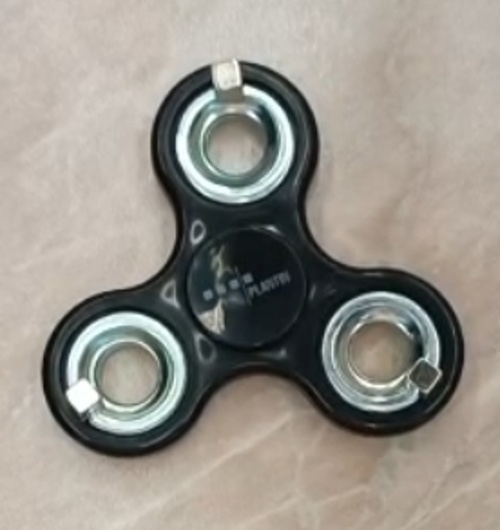
\includegraphics[width=0.3\textwidth]{osazeny_spinner.png}
    \centering
    \caption{Spinner osazený neodymovými magnety}
    \label{fig:1spinner}

    \vspace*{2.5cm}
    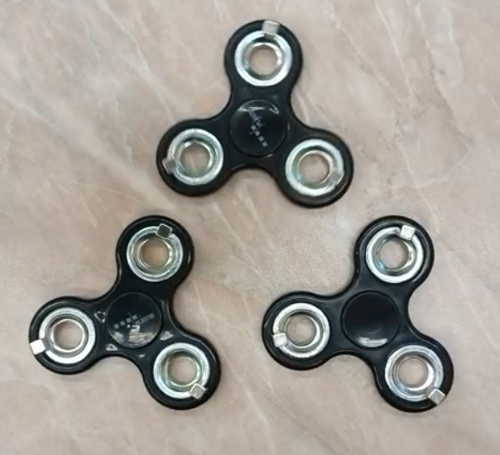
\includegraphics[width=0.35\textwidth]{3spinnery.png}
    \centering
    \caption{Tři interagující spinnery}
    \label{fig:3spinners}
\end{wrapfigure}

Prvním krokem v řešení této úlohy bylo kvalitativní sledování chování spinnerů v několika konfiguracích. Účelem tohoto bylo určení relevantních parametrů a seznámení se s problémem.

Hlavním poznatkem je, že dochází ke změně chování systému dvou spinnerů v závislosti na jejich relativních rychlostech.
Máme-li na stole 2 spinnery, ze kterých je jeden nehybný, a druhý roztočíme na nízkou rychlost, dojde po krátké chvíli k silné a chaotické interakci (záznam experimentu je k vidění v příloze \ref{attachment_1}).
Naopak, roztočíme-li druhý spinner znatelně rychleji, nedochází téměř k žádné interakci (viz příloha \ref{attachment_2}).
Druhý spinner se prvnímu spinneru efektivně jeví jako permanentí magnet - první spinner se tedy nanejvýše umístí do energeticky nejvýhodnější polohy a dále zůstává nehybný.
Dalším cenným poznatkem je, že při interakci více spinnerů se systém chová chaoticky téměř vždy (viz příloha \ref{attachment_3}).
Toto dělá měření interakcí více jak dvou spinnerů složité a za účelem získání použitelných výsledků omezéme náš výzkum pouze na jeden či dva spinnery.
Po vytvoření fyzikálního modelu pro popsání menšího počtu spinnerů se pokusíme o vývoj simulace, která by dovolila větší počty spinnerů.

Ze zadání můžeme také vyčíst další užitěčná omezení.
O umístění všech spinnerů je řečeno, že mají být v \textit{"(jedné) rovině vedle sebe"}. Dále má docházet k točení pouze \textit{"jedním z nich"} a interakce mezi spinnery mají probíhat pouze na bázi \textit{"vlivů magnetického pole"}.
Neměli bychom opomenout ani skutečnost, že všechny spinnery mají být \textit{"identické"}.
\clearpage

\section{Určení parametrů}

Z úvodního sledování není těžké určit relevantní parametry a vybrat, které z nich je možné s naším vybavením měřit. Vybranými parametry se budeme zabývat v následujících kapitolách.

\subsection{Parametry týkající se konfigurace spinnerů}
\label{sub:param_konf}
Jakožto nejdůležitější bychom určitě označili relativní pozice všech spinnerů, které popíšeme pomocí jejich středů $S_1, S_2,...$ (každý střed je braný jako vektor v rovině spinnerů) a jejich poloměrů $r_1, r_2, ...$.
Dále bude k přesnému určení pozic magnetů nezbytné znát okamžitý úhel rotace každého spinneru. Ty ozačíme $\varphi_1, \varphi_2,...$.
Nakonec k popsání spinneru musíme určit počet ramen (neboli počet připevněných magnetů). Tento počet označíme $n$. V našem případě je roven 3.

Pomocí těchto údajů je triviální vyjádřit pozici $P(i)$ libovolného magnetu jeho indexem $i$ (kde $0 \leq i < n$):

\begin{equation}
    \label{eq:magnet_pos}
    P(i) = S + \biggr(r\cos{\bigg(\varphi + \frac{2\pi i}{n}\bigg)},
    r\sin{\bigg(\varphi+\frac{2\pi i}{n}}\bigg), 0 \bigg)
\end{equation}

\begin{wrapfigure}{r}{0.4\textwidth}
    \vspace*{-0.5cm}
    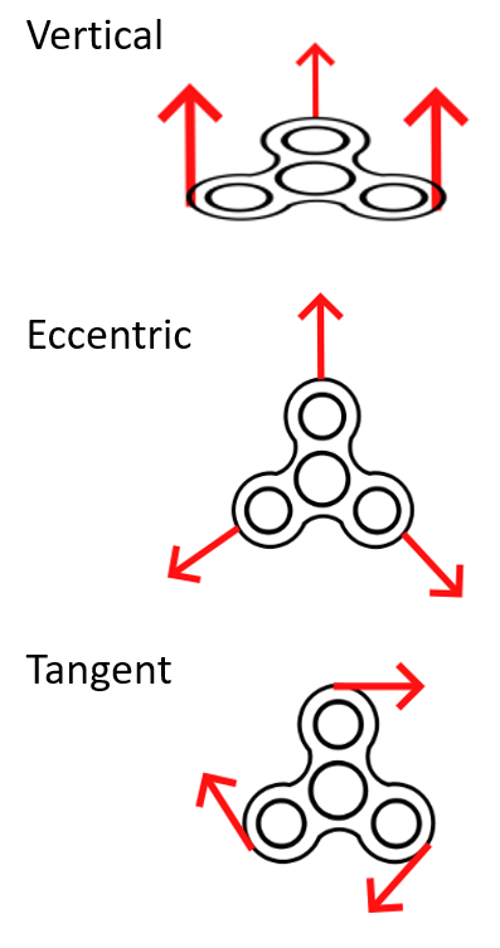
\includegraphics[width=0.3\textwidth]{orientace_magnetu.png}
    \centering
    \caption{Námi vyhrazené orientace magnetů}
    \label{fig:mag_orientations}
\end{wrapfigure}

Kromě pozice magnetu hraje také klíčovou roli nasměrování jeho pólů. Zde definujeme 3 důležité orientace (viz \autoref{fig:mag_orientations}):

\begin{enumerate}[topsep=0pt, partopsep=0pt]
    \setlength{\itemsep}{0pt}%
    \setlength{\parskip}{0pt}%
    \item \textbf{Vertikální (\textit{vertical})}
    \item Odstředivá (\textit{eccentric})
    \item Tečná (\textit{tangent})
\end{enumerate}

V našich experimentech jsme používali převážně vertikální konfiguraci, jelikož takto bylo uchycení magnetů nejjednodušší, protože se magnety samy připevnily ke kovovému závaží umístěnému v každém z ramen spinneru (viz \autoref{fig:1spinner}). Ta jsou zde za účelem zvýšení momentu setrvačnosti spinneru.

Tyto konfigurace jsme také schopni popsat, a to opět jakožto funkci indexu magnetu.
Nejdříve vyjádříme směrový vektor magnetického momentu $\vec{u}(i)$ pro $i$. magnet v každé konfiguraci (viz \autoref{tab:mag_dir_vec})

\vspace{24pt}

\begin{table}[!ht]
    \captionsetup{justification=raggedright,singlelinecheck=off}
    \caption{Směrové vektory pro různé konfigurace}
    \label{tab:mag_dir_vec}

    \def\arraystretch{1.5}
    \begin{tabularx}{\textwidth}{p{0.50\textwidth} p{0.50\textwidth} }
        \textbf{Konfigurace} & \textbf{Směrový vektor magnetu}                    \\
        \hline
        Vertikální           & $\vec{u}(i) = (0,0,1)$                             \\
        Odstředivá           & $\vec{u}(i) = \widehat{P(i) - S}$                  \\
        Tečná                & $\vec{u}(i) = (0,0,1) \times \widehat{(P(i) - S)}$ \\
    \end{tabularx}
\end{table}

{\raggedright
Když nyní zvolíme velikost magnetického momentu našich magnetů $|\vec{m}_0|$, jsme schopni popsat magnetický moment včetně jeho velikosti\footnote{Všimněme si, že $u(i) = \hat{u}(i)$.}:}

\begin{equation}
    \label{eq:magnet_moment_orientation}
    \vec{m} = |\vec{m}_0| \cdot \vec{u}(i)
\end{equation}

Velikost magnetických momentů bude záviset na teplotě, velikosti a materiálových vlastnostech magnetů (např. jejich chemickém složení a kvalitě). Ale to, jaká je pravá velikost magnetických momentů našich magnetů, je momentálně nepodstatné a určíme ji později (viz \autoref{sec:remanence_measurement}).

Posledním parametrem, který zmíníme v této části je, zda se magnety přitahují, či odpuzují.
V našem případě jsme se zaměřili na systémy, kde se všechny magnety odpuzují.

\subsection{Parametry týkající se pohybu spinnerů}
\label{sub:param_move}

Druhou, složitější, částí popisu našeho systému je jeho pohyb a chování v čase.
Zde se nevyhneme úhlovým rychlostem jednotlivých spinnerů, které budeme značit $\omega_1, \omega_2,...$.
Poté nás přirozeně zajímají i jejich úhlová zrychlení $\alpha_1, \alpha_2, ...$. Pro naše výpočty bude také často potřeba využít definice momentu síly a proto ji zmíníme. Definující závislost je následující: $\tau = I\alpha$ (kde $\tau$ značí moment síly a $I$ značí moment setrvačnosti\footnote{Někdy také značeno $J$.} spinneru).
Určení momentu setrvačnosti bude věnována vlastní kapitola (viz \autoref{sec:moment_of_inertia}).

Posledním dynamickým parametrem, který zmíníme, je tření v ložiscích spinnerů a jiné odporové síly působící na spinner.
Těm se budeme do hloubky věnovat v kapitole \ref{chap:drag}.

\clearpage

\section{Modelování magnetů}
V průběhu našich experimentů používáme neodymové (NdFeB) magnety krychlového tvaru o hraně 5mm a jakosti N35\footnote{Jakosti neodymových magnetů se pohybují od N35 do N55 \cite{magnet_grades}.}.
Toto standardní označení jakosti neodymových magnetů popisuje jejich chemické složení, tepelnou odolonost a hlavně magnetickou sílu \cite{magnet_grades}, která je popsána pomocí tzv. remanentní magnetizace, neboli remanence.

Jelikož jsou magnety poměrně malé, můžeme je ve větších vzdálenostech aproximovat jakožto magnetické dipóly.
Zároveň existuje velmi elegantní způsob, jak vypočítat velikost magnetického dipólu z jeho remanence \cite{magnetic_torque}:

\begin{equation}
    \label{eq:mag_mom_remanence}
    |\vec{m}_0| = \frac{1}{\mu_0}|\vec{B}_r|V
\end{equation}

Tabulkové hodnoty pro remanenci NdFeB magnetů jsou sice známé, ale v našem případě budeme přesnou hodnotu $|\vec{B}_r|$ našich magnetů měřit později, v kapitole \ref{sec:remanence_measurement}.

\section{Popis magnetických interakcí}

Jelikož k popisu magnetů používáme idealizaci pomocí magnetických dipólů, můžeme popsat interakce mezi nimi pomocí následujících rovnic.
Hlavní interakce mezi dvěma magnetickými dipóly jsou:
\begin{enumerate}[topsep=0pt, partopsep=0pt]
    \setlength{\itemsep}{0pt}%
    \setlength{\parskip}{0pt}%

    \item Silové interakce \cite{magnetic_force} mezi dvěma momenty $\vec{m}_1$ a $\vec{m}_2$, které jsou od sebe vzdáleny\footnote{$\vec{r} = P_1 - P_2$} $\vec{r}$:

          \begin{equation}
              \label{eq:F_m}
              \begin{split}
                  F_m (r,m_1,m_2) = \frac{3\mu_0}{4\pi ||r||^5}
                  \bigg[
                      (m_1\cdot r) m_2 +
                      (m_2\cdot r) m_1 +
                      (m_1\cdot m_2) r -
                      \frac{5(m_1\cdot r)(m_2\cdot r)}{||r||^2} r
                  \bigg] \\
              \end{split}
          \end{equation}

    \item Magnetické interakce, neboli působení momentu síly \cite{magnetic_torque} na $\vec{m}_2$ z důvodu vytvoření magnetického pole $B(r, m_1)$ momentem $\vec{m}_1$ \cite{magnetic_force}:

          \begin{equation}
              \label{eq:B}
              \begin{split}
                  B (r, m) = \frac{\mu_0}{4\pi}\frac{3 \hat{r}(\hat{r}\cdot m) - m}{|r|^3} \\
                  \tau = m_2 \times B(r, m_1)
              \end{split}
          \end{equation}
\end{enumerate}


\chapter{Měření parametrů}
\label{chap:param}

\begin{wrapfigure}{r}{0.5\textwidth}
    \vspace*{0.75cm}
    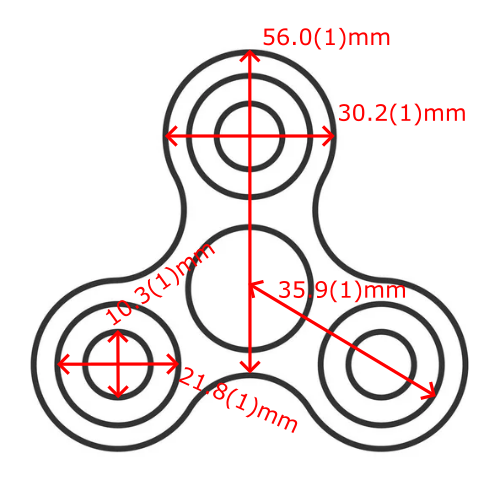
\includegraphics[width=0.45\textwidth]{dims.png}
    \centering
    \caption{Ilustrace spinneru společně s vyznačenými rozměry}
    \label{fig:spinner_size}
\end{wrapfigure}

\section{Rozměry spinneru}
\label{sec:spinner_size}
K popsání spinneru nejdříve určíme jeho rozměry (viz \autoref{fig:spinner_size}).
Nejdůležitější rozměr pro nás bude vzdálenost osy otáčení od místa, kde budou umístěny magnety.
To je v našem případě $r = 35.9(1)mm$.

Vzhledem k tomu, že na sebe spinnery mohou vzájemně působit pouze magnetickými silami, jak je řečeno v zadání, není třeba řešit zbytek geometrie spinneru v budoucích modelech.
Spinner budeme dále modelovat pouze jako $n$ magnetických dipólů, které se otáčejí kolem středu $S$ a pevně si udržují své relativní pozice.
Tomuto celkovému systému definujeme moment setrvačnosti podle následujícího měření.
\section{Moment setrvačnosti}
\label{sec:moment_of_inertia}
{\raggedright
    K určení momentu setrvačnosti spinneru bylo využito idealizace spinneru jakožto fyzického kyvadla, pro které platí: \cite{physical_pendulum}
}
\begin{equation}
    \label{eq:mag_pend}
    \omega = \sqrt{\frac{mgr}{I}}
\end{equation}
A po vyjádření z rovnice \ref{eq:mag_pend} získáváme:
\begin{equation}
    \label{eq:mom_inert}
    I = \frac{mgr}{\omega^2} = \frac{mgr}{4\pi^2f^2}
\end{equation}
Nyní stačí změřit frekvenci kmitů zavěšeného spinneru s několika magnety na jednom z jeho ramen a dopočítat moment setrvačnosti.

\begin{wrapfigure}{r}{0.5\textwidth}
    \vspace*{-0.75cm}
    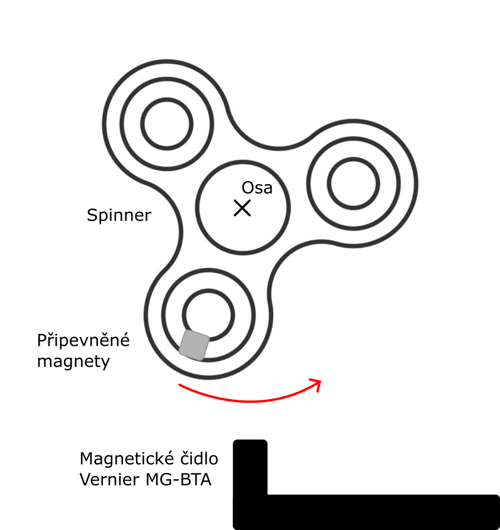
\includegraphics[width=0.45\textwidth]{mom_inert_setup.png}
    \centering
    \caption{Ilustrace aparatury pro měření frekvence kmitů spinneru}
    \label{fig:spinner_pendulum_aparature}
\end{wrapfigure}
\subsection{Aparatura}
Po připevnění šesti neodymových magnetů o jednotkové hmotnosti $0.92(1) g$ byl spinner připevněn pevně ve své ose otáčení.
Pod takto zavěšený spinner bylo umístěno magnetické čidlo Vernier MG-BTA, které zaznamenávalo, jak blízko se magnety nacházejí.
Po umístění spinneru mimo rovnovážnou polohu byl ponechán oscilovat a záznam průběhu magnetického pole v čase byl čidlem nasnímán (viz \autoref{fig:spinner_pendulum_recording}).
\vspace{40pt}

{\raggedright
    \subsection{Analýza měření a výsledky}
    Průběh následně analyzujeme pomocí programovacího jazyku \texttt{Python} \cite{python} a knihovny \texttt{scipy} \cite{scipy}.
    Námi kýžená maxima, která odpovídají půlperiodě kmitu, vyhledáme použitím funkce \texttt{scipy.signal.find\_peaks} a z jejich počtu jsme schopni určit počet period, kterými kyvadlo prošlo za určený čas.
}

\begin{wrapfigure}{r}{1\textwidth}
    \includegraphics[width=1\textwidth]{spin_pendulum_field_rec.png}
    \centering
    \caption[Nasnímaný průběh magnetické indukce v čase pro spinnerové kyvadlo]{Nasnímaný průběh magnetické indukce v čase (modře) pro spinnerové kyvadlo. Peaky, označující uplynutí jedné půlperiody, jsou vyznačeny červeně.}
    \label{fig:spinner_pendulum_recording}
\end{wrapfigure}

\clearpage

Máme-li tedy soubor \footnote{$|p|$ označuje počet prvků pole $p$; $p_{min}$ označuje čas prvního peaku; $p_{max}$ označuje čas posledního peaku.} $p$ všech časů nalezených peaků, je výpočet frekvence následující:
\begin{equation}
    \label{eq:freq_from_peaks}
    f = \frac{ |p| - 1}{2(p_{max} - p_{min})} = 1.00(1)Hz
\end{equation}

Dosazením do předchozí rovnice \ref{eq:mom_inert} získáváme výslednou hodnotu\footnote{Tato hodnota je srovnatelná s jinými zdroji dostupnými online (viz. \cite{spinner_mom_inert_external}).}:
\begin{equation}
    \label{eq:mom_inert_results}
    I = 4.80(50) \cdot 10^{-5} kg \cdot m^2
\end{equation}

\subsection{Popis skriptu}

V níže připnutém ústřižku kódu \ref{code:1} nejdříve načteme použité knihovny:
\texttt{numpy} \cite{numpy} pro provedení konvoluce,
\texttt{matplotlib} pro vytvoření grafu \ref{fig:spinner_pendulum_recording} \cite{matplotlib} a nakonec
\texttt{scipy}, kde využijeme funkce \texttt{find\_peaks}, jak již bylo zmíněno.

Prvním krokem je načtení dat ze souboru \texttt{kyvadlo.csv} a jejich převedení z textového formátu do 2D pole pojmenovaného \texttt{data}.
Dále izolujeme data jednotlivých os do separátních proměnných \texttt{xdata}, \texttt{ydata}.

\texttt{ydata} vyhladíme, abychom se zbavili šumu a to pomocí konvoluce použitím funkce \texttt{numpy.convolve}.
Délku 1D konvoluční matice jsme zvolili $m = 15$ a konvoluční matice délky $m$ by v našem případě obecně vypadala takto:

\begin{equation}
    \label{eq:conv_matrix_avg}
    M_{conv} =
    \underbrace{
        \begin{pmatrix}
            \frac{1}{m} & \frac{1}{m} & ... & \frac{1}{m}
        \end{pmatrix}
    }_{m\text{ krát}}
\end{equation}

Tato konvoluční matice provádí aritmetický průměr $m$ za sebou jdoucích hodnot.

Nyní provedeme hledání peaků na vyhlazených datech pomocí funkce \texttt{find\_peaks}, která akceptuje další dobrovolné argumenty:
\begin{enumerate}[topsep=0pt, partopsep=0pt]
    \setlength{\itemsep}{0pt}%
    \setlength{\parskip}{0pt}%
    \item height: určuje minimální absolutní velikost peaku
    \item threshold: minimální rozdíl dvou sousedních hodnot, aby bod mohl být peakem
    \item distance: minimální indexová vzdálensot dvou peaků
\end{enumerate}

Poté určíme časový interval, kde se peaky nacházejí (a přidáme na každou stranu 0.5 sekundy pro přehlednost grafu),
a vygrafujeme původní naměřená data (modře) společně s pozicemi peaků (červeně). Dále označíme osy.

Nakonec dopočítáme frekvenci kmitů kyvadla podle vzorce \ref{eq:freq_from_peaks} a vypíšeme ji.

\clearpage

\lstinputlisting[language=Python, caption=Kód k analyzování spinnerového kyvadla, label=code:1]{./prilohy/snippets/c1.py}

\section{Remanence $\vec{B}_r$}
\label{sec:remanence_measurement}

K určení remanence našich magnetů využijeme dvou různých metod. Jedna z nich bude založena na silové interakci magnetů a jedna na magnetem vytvořeném poli.

\subsection{Určení remanence přes magnetické pole}

Prvním způsobem, jak určit hodnotu remanentní magnetizace našich magnetů, je měření magnetického pole pomocí magnetometru mobilního telefonu.
Aplikace \texttt{Phyphox} umožňuje čtení těchto dat, která následně analyzujeme.

Měření provedeme pro sloupce 2 a 3 magnetů, abychom oveřili, zda je náš způsob měření konzistentní.
Dále také měříme větší neodymový magnet, jehož parametry nám nejsou známé, a který budeme používat v některých budoucích experimentech.
Abychom odstranili pozadí tvořené magnetickým polem země, provedeme měření magnetického pole magnetu v jedné orientaci a poté magnet otočíme a změříme hodnotu při opačné orientaci.
K získání výsledku jednoduše odečteme rozdíl naměřených hodnot, což bude dvojnásobek velikosti magnetického pole tvořeného magnetem.
Je zřejmé, že tímto odstraníme z meření jiné, neměnné, zdroje magnetických polí.

Kromě provádění měření pro různé počty a velikosti magnetů, budeme také meřit pole v různých vzdálenostech od magnetu, abychom dále potvrdili, zda je měření a náš model konzistetní.
Celkem provedeme tedy měření 2 magnetů, 3 magnetů a velkého magnetu pro vzdálenosti 5 cm, 10 cm, 20 cm a 30 cm.

\subsubsection{Analýza měření}
Výstupem aplikace \texttt{Phyphox} jsou sobory typu \texttt{.csv}, neboli \textit{"Comma separated values"} \cite{csv}.
Toto je poměrně čitelný a přívětivý formát ukládání dat, který v \texttt{Pythonovém} skriptu načteme pomocí funkce \texttt{open} (stejně jako v kódu \ref{code:1}).
Jinak budeme používat tyto knihovny:
\texttt{numpy},
\texttt{matplotlib} pro vytvoření grafu \ref{fig:mag_field_recording_2mag_10cm},
\texttt{scipy}, kde využijeme funkce \texttt{curve\_fit}, a
\texttt{math} \cite{pymath}.
Poté ručně určíme názvy všech datových souborů a časové intervaly, na kterých jsou magnety orientovány k snímači a od snímače.

Po načtení dat vyjmeme pouze hodnoty ve dříve zmíněných intervalech a najdeme jejich průměrnou hodnotu a odchylky.
Z rozdílu průměrných hodnot magnetického pole v obou otočeních magnetů určíme velikost magnetického pole generovaného pouze magnetem (očištěného od pozadí).
Z odchylek také určíme celkovou odchylku výsledné hodnoty.

Následně pro každé měření vytvoříme graf (příkladem je \autoref{fig:mag_field_recording_2mag_10cm}).

\lstinputlisting[language=Python, caption=Kód k určení průměrné hodnoty magnetického pole a odchylek, label=code:2]{./prilohy/snippets/c2.py}

\begin{wrapfigure}{c}{1\textwidth}
    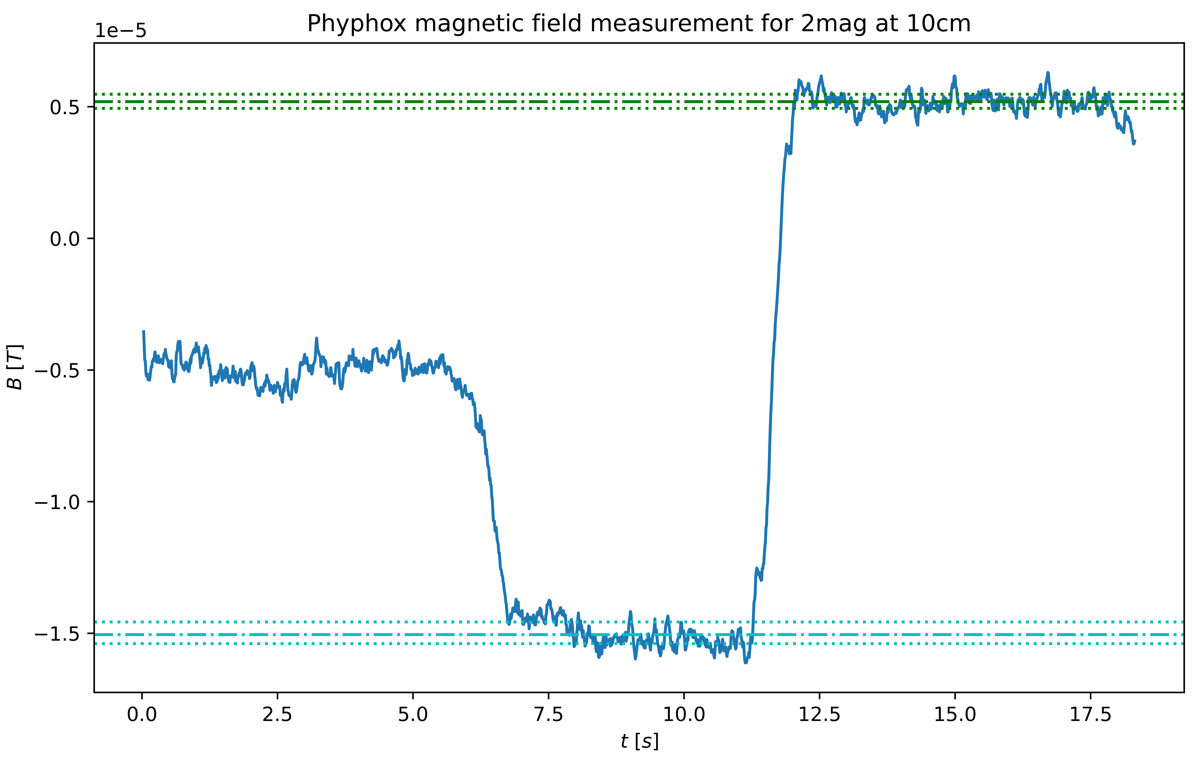
\includegraphics[width=1\textwidth]{mag_field_measurement_2mag_10cm.png}
    \centering
    \caption[Nasnímaný průběh magnetické indukce v čase pro účely měření remanence]{Nasnímaný průběh magnetické indukce v čase (modře) pro určení remanence. Průměrné hodnoty horní orientace (zeleně čerchovaně) a dolní orientace (modře čerchovaně). Odpovídající odchylky jsou znázorněny tečkovaně. Výsledná hodnota magnetické indukce tohoto příkladu, tedy dvou magnetů ve vzdálenosti 10 cm, je: $B = 1.01(8) \cdot 10^{-5} T$}
    \label{fig:mag_field_recording_2mag_10cm}
\end{wrapfigure}

\clearpage

Po zanalyzování všech měření můžeme vytvořit graf závislosti $B$ na vzdálenosti (viz \autoref{fig:B_in_dist}):

\begin{wrapfigure}{r}{0.5\textwidth}
    \vspace*{0.5cm}
    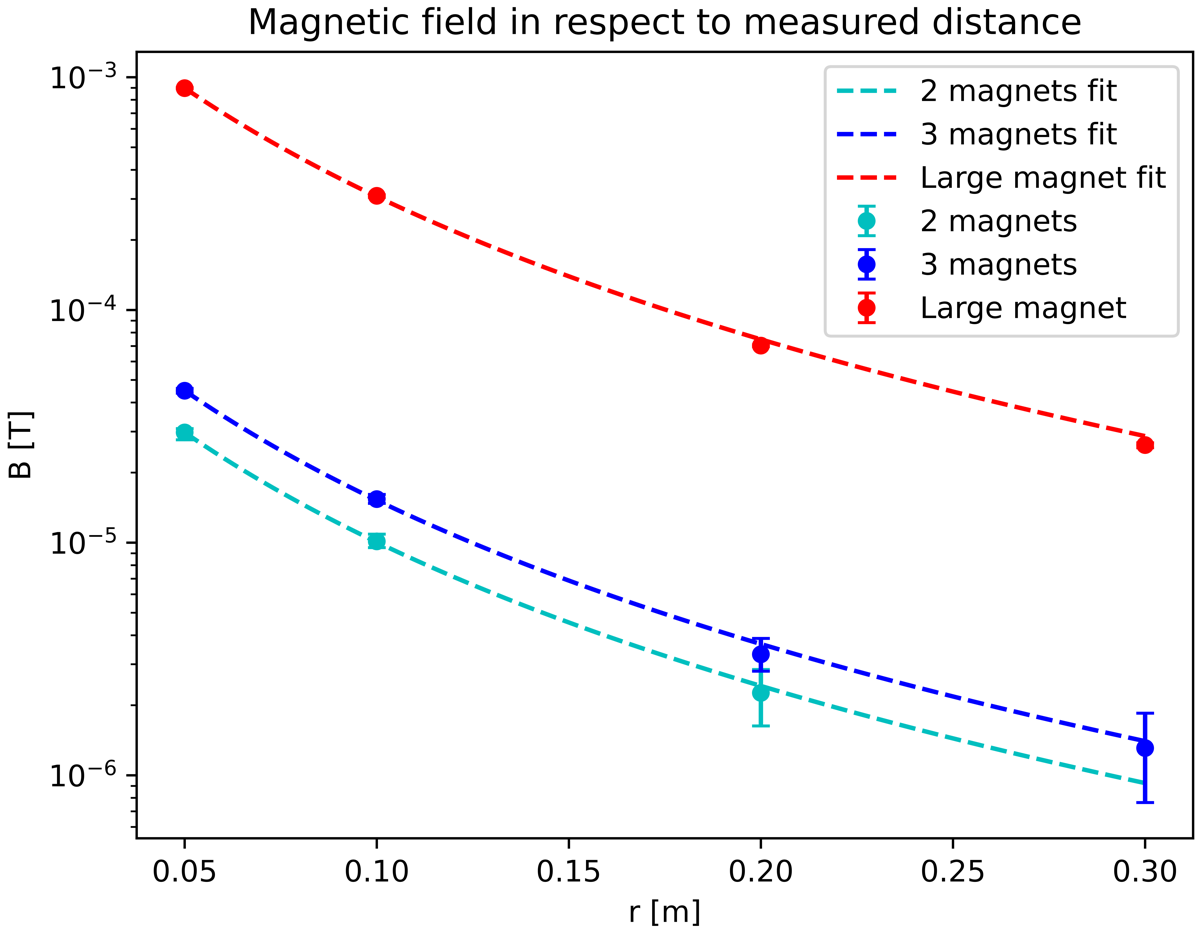
\includegraphics[width=0.45\textwidth]{B_field_in_distance.png}
    \centering
    \caption[Závislost magnetické indukce na vzdálenosti]{Závislost magnetické indukce na vzdálenosti. Sledujeme, že $B \propto r^{-3}$}
    \label{fig:B_in_dist}
\end{wrapfigure}

Pro určení $B_r$ z naměřených hodnot provedeme zjednodušení vzorce \ref{eq:B}, kdy nahradíme vektory pouze jejich velikostmi:

\begin{equation}
    \label{eq:B_reduced}
    |B| = \frac{{\mu}_0 |m|}{2\pi r^3}
\end{equation}

Zde si všímáme úměrnosti $B \propto r^{-3}$, kterou také sledujeme v našich naměřených datech.
Následným dosazením rovnice \ref{eq:mag_mom_remanence} a vyjádřením remanence získáváme:

\begin{equation}
    \label{eq:Br_from_B}
    |B_r| = \frac{2\pi r^3 |B|}{V}
\end{equation}

Pro každou naměřenou hodnotu $B$ dopočítáme odpovídající $B_r$ a výsledky zobrazíme v jednotném grafu \ref{fig:rem_final}.

\subsection{Určení remanence přes sílu}

Druhý způsob, kterým jsme schopni určit remanenci, je skrze přitahování (resp. odpuzování) jednoho magnetu k (resp. od) druhého magnetu. Posazením jednoho magnetu na váhu a sledováním změny měřené hmotnosti jsme z gravitačního zrychlení schopni dopočítat působící sílu druhého magnetu, který je umístěn v určité výšce. Zároveň první magnet podložíme lehkou, tlustou a nemagnetickou vrstvou (např. blokem polystyrenu), abychom zabránili interakci magnetu s kovovými částmi váhy.

\begin{wrapfigure}{r}{0.5\textwidth}
    \vspace*{-1cm}
    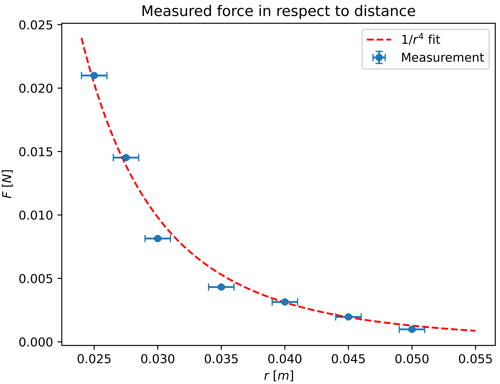
\includegraphics[width=0.45\textwidth]{F_in_distance.png}
    \centering
    \caption[Závislost magnetické síly na vzdálenosti]{Závislost magnetické síly na vzdálenosti. Sledujeme, že $F \propto r^{-4}$}
    \label{fig:mag_force_in_dist}
\end{wrapfigure}

Výhodou této metody je, že jsme schopni přesněji měřit slabší magnety, jelikož je můžeme dát blíže. V předchozí kapitole jsme nebyli schopni přiblížit magnety dostatečně blízko ke snímači telefonu kvůli jeho rozměrům.
Toto měření provádíme pouze pro 1 magnet, jelikož pro ten nám chybí výsledky z měření pomocí magnetického pole (ze dříve zmíněných důvodů). Výsledky můžeme vidět na grafu \ref{fig:mag_force_in_dist}.

\clearpage

Výpočet remanence provedeme podobně jako u rovnice \ref{eq:B_reduced} a to náhradou vektorů za jejich velikosti v rovnici \ref{eq:F_m}. Tím jsme ji schopni zjednodušit na následující podobu:

\begin{equation}
    \label{eq:F_reduced}
    |F| =  \frac{3 {\mu}_0}{2\pi r^4}|m|^2
\end{equation}

Po dosazení rovnice \ref{eq:mag_mom_remanence} a vyjádřením remanence získáváme:

\begin{equation}
    \label{eq:Br_from_F}
    B_r = \sqrt{\frac{2\pi {\mu}_0 r^4 F}{3 V^2}}
\end{equation}

Výsledné hodnoty $B_r$ zobrazíme v jednotném grafu \ref{fig:rem_final}.

\subsection{Výsledky}

Výsledky obou způsobů měření sjednotíme do grafu závislosti $B_r$ na vzdálenosti (viz \autoref{fig:rem_final}).
Očekávali bychom, že se $B_r$ v závislosti na vzdálenosti nebude měnit, a pro každé měření určíme pomocí optimalizace fitu konstantní funkcí souhrnnou hodnotu. Výsledkem všech měření bude aritmetický průměr těchto souhrnných hodnot.

\begin{wrapfigure}{r}{0.5\textwidth}
    \vspace*{-0.5cm}
    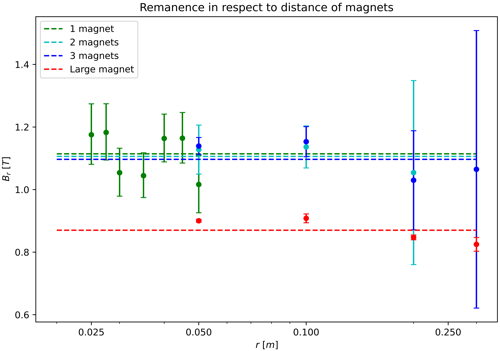
\includegraphics[width=0.5\textwidth]{Final_remanence.png}
    \centering
    \caption[Souhrnný graf všech měření remanence]{Souhrnný graf všech měření remanence. Ve výpočtu výsledné hodnoty $B_r$ není započítávána remanence velkého magnetu, jelikož není součástí stejné várky magnetů a budeme s ním nakládat později jinak.}
    \label{fig:rem_final}
\end{wrapfigure}

Výsledná hodnota remanence našich krychlových magnetů je \footnote{Námi naměřené hodnoty jsou srovnatelné s externími zdroji (viz. \cite{magnet_grades}).}:
$$
    B_r = 1.10(13) T
$$

a našeho velkého magnetu je:
$$
    B_{r_{xl}} = 0.87(5)T
$$

Důvodem, proč je remanence většího magnetu znatelně nižší, může být skutečnost, že takto velký magnet náš model není schopen popsat jako jediný magnetický dipól, nebo například jeho stáří.

\clearpage

\chapter{Tření}
\label{chap:drag}

O třecích jevech při otáčení spinneru jsme si již byli schopni udělat představu při úvodním kvalitativním sledování. Tření bude hrát značnou roli v našem systému, protože právě tření bude hlavním limitujícím faktorem průběhu chaotického chování. Dalším využitím, kromě našeho hlavního záměru - zpřesnění popisu chování, bude také například možnost odhadnutí maximálního času, než systém ztratí všechnu svou energii. Zajímavým a snadno měřitelným pro nás bude průběh úhlové rychlosti $\omega$ v čase (resp. změna úhlové rychlosti\footnote{$I\dot{\omega} = \tau$}), ze kterého vyplývá i náš popis těchto třecích složek.

Zajímá-li nás tedy změna rychlosti, dovolíme si odhadnout, že hlavními zdroji tření bude ložisko a odpor vzduchu. Provedeme idealizaci ložiska a řekneme, že jeho brzdný moment síly, a tím pádem i úhlové zpomalení, bude neměnné v čase a nezávislé na rychlosti. Toto nemusí být vždy pravda - například objeví-li se v reálném ložisku nějaké nechtěnné oscilace (které jsme sledovali) nebo je-li na ložisko působeno nějakou externí silou mířící kolmo na osu otáčením (jako například když se od sebe velmi silně odpuzují magnety ze dvou blízkých spinnerů). Oba tyto příklady jsou příliš složité k popsání a nejsme je tedy schopni zkoumat. Toto brzdné úhlové zrychlení (resp. zpomalení) nezávislé na rychlosti spinneru označíme $\alpha$.

Další výraznou složkou bude již zmíněný odpor vzduchu. Z látky středoškolské fyziky známe přibližnou úměrnost odporové síly na kvadrátu rychlosti ($F \propto v^2$) při turbulentním proudění (které v našem případě očekáváme kvůli složité geometrii spinneru). Při rotaci spinneru bychom tedy analogicky očekávali proporcionalitu $\dot{\omega} \propto \omega^2$. Míru této závislosti označíme $\gamma$.

Poslední složkou, pro kterou nejsme schopni najít fyzikální podstatu, ale kterou přesto budeme zkoumat je lineární složka $\beta$. Existují-li tedy jevy, které nám unikly, a platí pro ně závislost $\dot{\omega} \propto \omega$, můžeme je kompenzovat touto složkou. Zároveň budeme podrobně srovnávat přesnosti našich předpokladů včetně, ale i bez, této složky, abychom určili, zda dává smysl tuto složku využívat.

\clearpage

\section{Analytický popis}

Všechny tři dříve zmíněné složky dohromady tedy popisuje řídící závislost systému:\footnote{Záporná znaménka používáme čistě z toho důvodu, aby nám koeficienty $\alpha$, $\beta$ a $\gamma$ vycházely kladně, jelikož očekáváme, že systém bude zpomalovat.}:
\begin{equation}
    \label{eq:drag_diff_wlin}
    \dot{\omega}(t) = - \alpha - \beta \omega(t) - \gamma \omega^2(t)
\end{equation}

Pokud bychom odstranili lineární komponent, získáváme:
\begin{equation}
    \label{eq:drag_diff}
    \dot{\omega}(t) = - \alpha - \gamma \omega^2(t)
\end{equation}

Obě tyto diferencialní rovnice jsou analyticky řešitelné a jejich řešení pro $\omega$ jsou v totožném pořadí\footnote{Všimněme si, že rovnice \ref{eq:drag_res_wlin} je ekvivalentní rovnici \ref{eq:drag_res}, když $\beta = 0$.}:
\begin{equation}
    \label{eq:drag_res_wlin}
    \omega(t) = -\frac{\sqrt{4\alpha\gamma - \beta^2} \tan{(\frac{1}{2}\sqrt{4\alpha\gamma - \beta^2}(t-c_1)})-\beta}{2\gamma}
\end{equation}
a
\begin{equation}
    \label{eq:drag_res}
    \omega(t) = -\sqrt{\frac{\alpha}{\gamma}} \tan{(\sqrt{\alpha\gamma}(t-c_1))}
\end{equation}

\subsection{Maximální doba otáčení}

Parametr $c_1$\footnote{Někdy také označujeme $t_{max}$.} je hodnota v sekundách, která odpovídá době, po které se spinner zastaví. Vyjádřením $c_1$ (např. z druhé rovnice) jsme schopni určit poměrně přesně, jak dlouho se bude spinner točit, známe-li jeho parametry $\alpha$, ($\beta$) a $\gamma$ a jeho počáteční úhlovou rychlost $\omega_0$:
\begin{equation}
    \label{eq:runtime_from_omeg0}
    c_1(\omega_0) = \frac{1}{\sqrt{\alpha\gamma}} \arctan{ \bigg( \sqrt{\frac{\gamma}{\alpha}} \omega_0 \bigg)}
\end{equation}

Pokud bychom si přáli vyjádřit celkovou dobu otáčení z počáteční kinetické energie, můžeme dosadit $E_k = \frac{1}{2}I\omega^2$, kde je nám $I$ již známé (viz \autoref{sec:moment_of_inertia}), a jednoduchou úpravou získáváme:
\begin{equation}
    \label{eq:runtime_from_ene}
    c_1(E) = \frac{1}{\sqrt{\alpha\gamma}} \arctan{ \bigg( \sqrt{\frac{2 \gamma E}{\alpha I}} \bigg)}
\end{equation}

Jakmile dojde k tomu, že $t > c_1$, nepopisuje již funkce náš spinner, protože by začal opět nabývat energii a otáčet se opačným směrem, k čemuž nemůže dojít.

\clearpage

\subsubsection{Horní limit doby otáčení $n$ spinnerů}

Další zajímavou vlastností, kterou jsme schopni pro tento idealizovaný systém dokázat je, že máme-li libovolné (přirozené) množství spinnerů o počátečních energiích $E_1, E_2 ... E_n$, které spolu neinteragují, je maximální dobou $t_{max}$, po kterou se může některý z nich otáčet $t_{max} \leq c_1(\sum_{i=1}^n E_i)$. Tento fakt se může zdát triviálním a zbytečným, ale tímto způsobem jsme schopni určit například horní časovou hranici, po kterou by musela běžet simulace, než bychom si byli poměrně\footnote{Nemůžeme si být kompletně jisti kvůli interakcím spinnerů a nepřestnostem simulace.} jisti, že již došlo k zastavení všech spinnerů.

Pokud bychom chtěli zlepšit tento odhad i pro interagující spinnery, bylo by potřeba počítat s tím, že spinnery se mohou zrychlovat, zpomalovat a často budou oscilovat. Pokud bychom sledovali mnoho přibližně harmonických oscilací spinnerů, kdy se po relativně dlouhou dobu nepohybují svou nejvyšší rychlostí, mohli bychom se inspirovat efektivní hodnotou sinusoidy a udělat tak hrubý odhad, že $t_{max} \leq \sqrt{2} c_1(\sum_{i=1}^n E_i)$. Nad tím, jaká konstanta by byla dobrá, můžeme dlouze polemizovat, ale to není zájmem této práce, proto nebudeme myšlenku dále rozvádět.

Tuto vložku zakončíme důkazem dříve vyslovené věty, že $t_{max} \leq c_1(\sum_{i=1}^n E_i)$:

Nejdříve zdůrazníme několik zřejmých skutečností o naší funkci $c_1(E)$:

\begin{equation}
    \label{eq:max_runtime_proof_p1}
    \begin{gathered}
        c_1(E) = \frac{1}{\sqrt{\alpha\gamma}} \arctan{ \bigg( \sqrt{\frac{2 \gamma E}{\alpha I}} \bigg)} \\
        c_1(E) \text{ je rostoucí a prostá funkce pro } \alpha, \gamma \in \mathbb{R}^+ \\
        E_1, E_2, ..., E_n \in \mathbb{R}^+ \implies c_1(E_1), ..., c_1(E_n) \in \mathbb{R}^+
    \end{gathered}
\end{equation}

Bez újmy na obecnosti poté můžeme řící, že:
\begin{equation}
    \label{eq:max_runtime_proof_p2}
    \begin{gathered}
        E_1 \leq E_2 \leq ... \leq E_n \in \mathbb{R}^+ \implies c_1(E_1) \leq ... \leq c_1(E_n) \in \mathbb{R}^+
    \end{gathered}
\end{equation}

A obecně vybereme energie $E_u$ a $E_v$ takové, že $E_u \geq E_v$ ($u \neq v \wedge 1 \leq v < u \leq n$), pro které se snažíme dokázat následující:

\begin{equation}
    \label{eq:max_runtime_proof_p3}
    \begin{gathered}
        c_1(E_u+E_v) \stackrel{?}{\geq} \max(c_1(E_u), c_1(E_v)) \\
    \end{gathered}
\end{equation}

\clearpage

\subsubsection{Důkaz}
\begin{equation}
    \label{eq:max_runtime_proof_p4}
    \begin{gathered}
        c_1(E_u+E_v) \geq \max(c_1(E_u), c_1(E_v)) \\
        \\
        c_1(E_u+E_v) \geq \max(c_1(E_u), c_1(E_v)) \equiv c_1(E_u+E_v) \geq c_1(E_u) \because (c_1(E_u)\geq c_1(E_v) \because E_u \geq E_v) \\
        \\
        c_1(E_u+E_v) \geq c_1(E_u) \\
        \frac{1}{\sqrt{\alpha\gamma}} \arctan{ \bigg( \sqrt{\frac{2 \gamma (E_u+E_v)}{\alpha I}} \bigg)} \geq \frac{1}{\sqrt{\alpha\gamma}} \arctan{ \bigg( \sqrt{\frac{2 \gamma E_u}{\alpha I}} \bigg)} \\
        \arctan{ \bigg( \sqrt{\frac{2 \gamma (E_u+E_v)}{\alpha I}} \bigg)} \geq \arctan{ \bigg( \sqrt{\frac{2 \gamma E_u}{\alpha I}} \bigg)} \\
        \sqrt{\frac{2 \gamma (E_u+E_v)}{\alpha I}} \geq \sqrt{\frac{2 \gamma E_u}{\alpha I}}\\
        \sqrt{\frac{2 \gamma }{\alpha I}} \sqrt{E_u+E_v} \geq \sqrt{\frac{2 \gamma}{\alpha I}} \sqrt{E_u}\\
        \sqrt{E_u+E_v} \geq \sqrt{E_u}\\
        E_u+E_v \geq E_u\\
        E_v \geq 0\\
        \text{QED}
    \end{gathered}
\end{equation}

Dále pouhou analogií pro libovolné dvojice, větší $k$-tice a konečně celou $n$-tici energií je zřejmé, že:
\begin{equation}
    \label{eq:max_runtime_proof_p5}
    \begin{gathered}
        \forall E_j; (1 \leq j \leq n): c_1(E_j) \leq c_1 \Bigg(\sum_{i=1}^n E_i \Bigg) \\
        \Updownarrow \\
        t_{max} \leq c_1 \Bigg(\sum_{i=1}^n E_i \Bigg) \\
        \text{QED}
    \end{gathered}
\end{equation}

\subsection{Určení jednotek parametrů $\alpha$, $\beta$ a $\gamma$}

Přepsáním rovnice \ref{eq:drag_diff_wlin} pouze pomocí jednotek jsme schopni jednoduše odvodit jednotky koeficientů $\alpha$, $\beta$ a $\gamma$:
\begin{equation}
    \label{eq:drag_units}
    \begin{gathered}
        [rad \cdot s^{-2}] = - [\alpha] - [\beta] [rad \cdot s{-1}] - [\gamma] [rad \cdot s]^2 \\
        [rad \cdot s^{-2}] = - [rad \cdot s^{-2}] - [s^{-1}] [rad \cdot s{-1}] - [rad^{-1}] [rad^2 \cdot s^{-2}] \\
        \implies [\alpha] = [rad \cdot s^{-2}]; [\beta] = [s^{-1}]; [\gamma] = [rad^{-1}]
    \end{gathered}
\end{equation}

\clearpage

\subsection{Experiment pro potvrzení analytického řešení}

Abychom ověřili, zda výsledky našich diferencialních rovnic odpovídají realitě, provedeme měření, kde budeme sledovat jak se snižuje úhlová rychlost každého z našich spinnerů v čase. K tomu využijeme opět magnetického čidla Vernier MG-BTA, které bude sledovat momenty, kdy se kolem něj mihne jeden z magnetů připevněných na ramenou spinneru (velmi podobně jako u \autoref{fig:spinner_pendulum_aparature}). Časová hustota těchto vrcholů je úměrná úhlové rychlosti - přesněji 1 vrchol za sekundu se rovná $\frac{2}{3}\pi$ $rad/s$.

\begin{wrapfigure}{r}{0.5\textwidth}
    \vspace*{-1.5cm}
    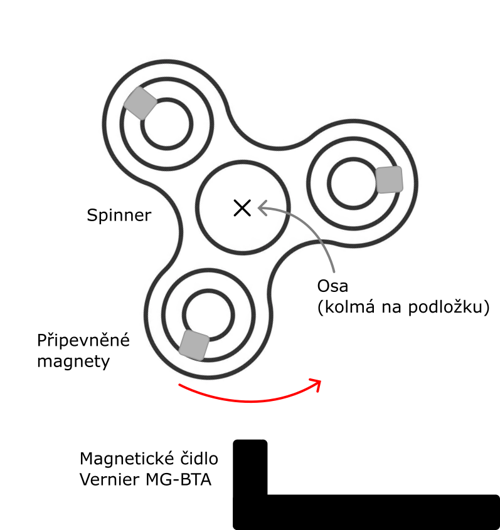
\includegraphics[width=0.45\textwidth]{drag_setup.png}
    \centering
    \caption{Ilustrace aparatury pro měření přibližné úhlové rychlosti spinneru}
    \label{fig:spinner_drag_aparature}
\end{wrapfigure}

\subsubsection{Aparatura}
Aparatura tohoto experimetu (vyobrazená na \autoref{fig:spinner_drag_aparature}) je velmi podobná té na \autoref{fig:spinner_pendulum_aparature}. Jediným rozdílem je, že nyní má spinner osazená všechna ramena a to pouze jedním magentem. Zároveň není zavěšen ve své ose, ale leží na podložce a je tedy jeho osa otáčení kolmá na prodložku (resp. rovnoběžná se směrem gravitačního zrychlení). V této orientaci budou prováděna i všechna následující měření v dalších kapitolách.

\begin{wrapfigure}{r}{0.5\textwidth}
    \vspace*{3cm}
    \includegraphics[width=0.5\textwidth]{peak_find_alg_drawing.png}
    \centering
    \caption{Ilustrace fungování algoritmu pro hledání peaků}
    \label{fig:peak_find_alg_drawing}
\end{wrapfigure}
\subsubsection{Zpracování dat}
Ke zpracování dat opět použijeme jazyk \texttt{Python} a stejné knihovny jako doposud.
Prvním úkolem je převedení průběhů kmitů magnetického pole (způsobených mihnutím magnetu před čidlem) do průběhu úhlové rychlosti v čase.
K tomto bude potřeba určit peaky a jejich pozici v čase a následně konvolucí počítat množství peaků na určitých intervalech.
Pozice peaků určíme tak, že budeme sledovat kdy naměřená hodnota překročí nějaký práh. Toto bude začátek našeho peaku.
Když půjde zpět pod hodnotu prahu, ukončíme peak. Pozici maxima umístíme do středu tohoto časového intervalu (viz \autoref{fig:peak_find_alg_drawing}).

\clearpage
\lstinputlisting[language=Python, caption=Kód k hledání pozic peaků, label=code:3]{./prilohy/snippets/c3.py}
Druhým krokem je projít celou časovou domému měření a rozdělit ji na menší intervaly. V těchto intervalech spočítáme počet peaků a přepočtem $1$ $peak/s = \frac{2\pi}{3}$ $rad/s$ určíme přibližnou průměrnou rychlost v tomto okolí.

\clearpage
\lstinputlisting[language=Python, caption=Pokračování kódu \ref{code:3} - výpočet úhlové rychlosti pomocí konvoluce, label=code:4]{./prilohy/snippets/c4.py}

\subsection{Výsledky a porovnání se simulací}
Po analýze všech naměřených dat výše uvedeným algorimem (celkem 7 měření, protože máme 7 různých spinnerů) a provedením fitu funkcí dle rovnice \ref{eq:drag_res_wlin} získáváme koeficienty v následucících rozmezích:
\begin{equation}
    \label{eq:drag_coef_res}
    \begin{gathered}
        0.220 \leq \alpha \leq 0.927 \\
        0.0 \cdot 10^{-15} \leq \beta \leq 2.5 \cdot 10^{-3} \\
        2.22 \cdot 10^{-4} \leq \gamma \leq 3.17 \cdot 10^{-4} \\
    \end{gathered}
\end{equation}

\subsection{Zhodnocení použití lineárního koeficientu}

\begin{wrapfigure}{r}{0.6\textwidth}
    \vspace*{0cm}
    \includegraphics[width=0.6\textwidth]{spinner_decay_with_beta.png}
    \centering
    \caption[Příklad grafu měřeného průběhu $\omega$ v $t$ s $\beta \neq 0$]{Příklad grafu měřeného průběhu úhlové rychlosti v čase (zeleně) v porovnání s fitem užívajícím všech tří brzdných složek (červeně). Simulace modře.}
    \label{fig:drag_fit_wlin}
\end{wrapfigure}

Nyní je na řadě prozkoumání významu a užitečnosti lineárního brzdného koeficientu. Získané hodnoty $\beta$ z předchozích sedmi měření nejsou konzistetní mezi spinnery, což je prvním indikátorem toho, že lineární složka nebude součástí dobrého popisu tření (alespoň pro tento případ).

Fitujeme-li stejná data funkcí bez lineární složky získáváme graf \ref{fig:drag_fit}. Vidíme, že simulace (jejíž implementací se budeme zabývat v \autoref{chap:sim}) v tomto případě lépe předpovídá měřené hodnoty.
\begin{wrapfigure}{r}{1\textwidth}
    \includegraphics[width=1\textwidth]{spinner_decay.png}
    \centering
    \caption[Příklad grafu měřeného průběhu $\omega$ v $t$ s $\beta = 0$]{Příklad grafu měřeného průběhu úhlové rychlosti v čase (zeleně) v porovnání s fitem užívajícím pouze složek $\alpha$ a $\gamma$ (červeně). Simulace modře.}
    \label{fig:drag_fit}
\end{wrapfigure}

\clearpage

Poslední měření, které jsme k účelům porovnání těchto dvou metod provedli, bylo sledování průběhu úhlové rychlosti, když byl spinner umístěn do magnetického pole našeho velkého magnetu. Velký magnet jsme upevnili 8cm od středu spinneru a stejnou aparaturou jako v minulém experimentu jsme sledovali jeho chování. Zde jsme prováděli pouze jedno měření a fitovali jsme ho opět oběma způsoby, které porovnáváme níže:
\begin{figure}[H]
    \includegraphics[width=0.65\textwidth]{sim_spinner_magnetic_with_beta.png}
    \centering
    \caption[Příklad grafu měřeného průběhu $\omega$ v $t$ s $\beta \neq 0$ v magnetickém poli]{Graf měřeného úhlové rychlosti v čase v porovnání s fitem užívajícím všech tří složek. (barevné schéma jako v \autoref{fig:drag_fit_wlin})}
    \label{fig:drag_fit_mag_wlin}
\end{figure}
Jak můžeme vidět na \autoref{fig:drag_fit_mag_wlin}, koeficient $\beta$ nám vychází efektivně nulový a průběhy fitů se od sebe téměř neliší.
Z těchto měření tedy ověřujeme naši předchozí představu, že lineární komponent tření není fyzikálně signifikantní.
\begin{figure}[H]
    \includegraphics[width=0.65\textwidth]{sim_spinner_magnetic.png}
    \centering
    \caption[Příklad grafu měřeného průběhu $\omega$ v $t$ s $\beta = 0$ v magnetickém poli]{Graf měřeného úhlové rychlosti v čase v porovnání s fitem užívajícím složek $\alpha$ a $\gamma$. (barevné schéma jako v \autoref{fig:drag_fit})}
    \label{fig:drag_fit_mag}
\end{figure}

\chapter{Simulace}
\label{chap:sim}

Jak již bylo zmíněno v předchozí kapitole a jak vychází z názvu této práce, značnou částí našeho zkoumání bylo také počítačové simulování těchto systémů.

\section{Popis způsobu simulování}

Naším cílem bude vytvoření tzv. \textit{"Discrete event simulation"} neboli \textit{DES} \cite{sim_methods}. Jedná se o druh simulační metody, která popisuje náš stav pomocí diskrétních stavů, které existují v daném čase. Z jednoho určitého stavu poté pomocí určitých pravidel popisujících náš systém simulační algoritmus provádí odhad toho, jak bude vypadat další stav po uplynutí $\Delta t$ sekund, kde $\Delta t$ je velmi malé. Toto nazveme nejdím simulačním krokem. Poté stačí opakovat simulační kroky dle libosti.

\subsection{Runge-Kutta metody}

Runge-Kutta metody, pojmenované po Carlu Davidu Tolmé Rungeovi a Martinu Wilhelmu Kuttovi, jsou rodinou metod používaných k řešení implicitních a explicitních diferenciálních rovnic. Implicitní metody popisující budoucí stav systému z předchozího stavu, stejně jak budeme dělat my v naší \textit{DES}. Runge-Kutta metody (také ornačované pouze RK metody) jsou tedy ideálním nástrojem pro simulování našeho problému. nejjednodušším příkladem RK metody je například Eulerova metoda. Těchto metod je nespočet, ale jejich obecný předpis je následující \cite{RK_def}:
\begin{equation}
    \label{eq:RK_def}
    \begin{gathered}
        y_{n+1} = y_n + \Delta t \sum_{i=1}^{s} b_i k_i \\
        k_m = f \Bigg(t_n + c_m \Delta t, y_n + \Bigg(\sum_{j=1}^{s-1} k_j a_{m,j} \Bigg) \Delta t \Bigg)
    \end{gathered}
\end{equation}

V tomto předpisu jednotlivé znamenají: $t_n$ je čas stavu $y_n$ a $\Delta t$ je krátký časový krok; $s$ je stupeň RK metody; $a_{m,j}$, $b_i$ a $c_m$ jsou specifické koeficinty dané RK metody; $y_n$ je stávající stav a $y_{n+1}$ je budoucí, předpovídaný, stav; $k_m$ je pomocný sub-stav; $f(t,y) = \dot{y}$.

Specifick0 koeficienty se nejčastěji zapisují pomocí tzv. Butcherových tabulek \cite{Butcher_tab_def} (pojmenovaných po Johnu Charlesovi Butcherovi). Zápis obecné Butcherovy tabulky pro RK metodu $s$. stupně je:
\begin{table}[!ht]
    \centering
    \captionsetup{singlelinecheck=off}
    \caption{Zápis obecné Butcherovy tabulky pro RK metodu $s$. stupně}
    \label{tab:Butch_tab}

    \begin{tabularx}{7cm}{c | c c c c c}
        $c_1 = 0$                                                            \\
        $c_2$    & $a_{2, 1}$                                                \\
        $c_3$    & $a_{3, 1}$ & $a_{3, 2}$                                   \\
        $\vdots$ & $\vdots$   &            & $\ddots$                        \\
        $c_s$    & $a_{s, 1}$ & $a_{s, 2}$ & $\cdots$ & $a_{s, s-1}$         \\
        \hline
                 & $b_1$      & $b_2$      & $\cdots$ & $b_{s-1}$    & $b_s$ \\
    \end{tabularx}
\end{table}

Některé z podmínek, které sice nezaručují konzistentnost a stabilitu metody, ale dobrými základními pravidly jsou \cite{Butcher_tab_def}:

\begin{equation}
    \label{eq:RK_conditions}
    \begin{gathered}
        \text{1)} \quad \quad \qquad \qquad \sum_{i=1}^{s} b_i = 1 \qquad \qquad \\
        \text{2)} \quad \quad \sum_{j=1}^{i-1} a_{i,j} = c_i \quad (i \in \{2,...,s\})
    \end{gathered}
\end{equation}

Níže vypíšeme Butcherovy tabulky několika základních metod, které byly později implementovány v simulaci \cite{RK_methods_list}:

\begin{table}[H]
    \parbox{.45\linewidth}{
        \centering
        \caption[Butcherova tabulka Eulerovy metody]{\textbf{Eulerova metoda}}
        \begin{tabular}{c | c}
            0 &   \\
            \hline
              & 1 \\
        \end{tabular}
    }
    \hfill
    \parbox{.45\linewidth}{
        \centering
        \caption[Butcherova tabulka metody středního bodu]{Metoda středního bodu}
        \begin{tabular}{c | c c}
            0   &         \\
            1/2 & 1/2     \\
            \hline
                & 0   & 1 \\
        \end{tabular}
    }
\end{table}
\begin{table}[H]
    \parbox{.3\linewidth}{
        \centering
        \caption[Butcherova tabulka Heunovy metody]{Heunova metoda}
        \begin{tabular}{c | c c}
            0 &           \\
            1 & 1         \\
            \hline
              & 1/2 & 1/2 \\
        \end{tabular}
    }
    \hfill
    \parbox{.3\linewidth}{
        \centering
        \caption[Butcherova tabulka Ralstonovy metody]{Ralstonova metoda}
        \begin{tabular}{c | c c}
            0   &           \\
            2/3 & 2/3       \\
            \hline
                & 1/4 & 3/4 \\
        \end{tabular}
    }
    \hfill
    \parbox{.3\linewidth}{
        \centering
        \caption[Butcherova tabulka obecné metody 2. stupně]{Obecná metoda 2. stupně}
        \begin{tabular}{c | c c}
            0        &                                               \\
            $\alpha$ & $\alpha$                                      \\
            \hline
                     & $1 - \frac{1}{2\alpha}$ & $\frac{1}{2\alpha}$ \\
        \end{tabular}
    }
\end{table}

\begin{table}[H]
    \parbox{.45\linewidth}{
        \centering
        \caption[Butcherova tabulka Simpsonova pravidla 3/8]{Simpsonovo pravidlo 3/8}
        \begin{tabular}{c | c c c c c}
            0   &                        \\
            1/3 & 1/3                    \\
            2/3 & -1/3 & 1               \\
            1   & 1    & -1  & 1         \\
            \hline
                & 1/8  & 3/8 & 3/8 & 1/8 \\
        \end{tabular}
    }
    \hfill
    \parbox{.45\linewidth}{
        \centering
        \caption[Butcherova tabulka RK4]{\textbf{Standardní Runge-Kutta metoda 4. stupně (neboli RK4)}}
        \begin{tabular}{c | c c c c c}
            0   &                       \\
            1/2 & 1/2                   \\
            1/2 & 0   & 1/2             \\
            1   & 0   & 0   & 1         \\
            \hline
                & 1/6 & 2/6 & 2/6 & 1/6 \\
        \end{tabular}
    }
\end{table}

\begin{table}[H]
    \hfill
    \parbox{.8\linewidth}{
        \centering
        \caption[Butcherova tabulka Ralstonovy metody 4. stupně]{Ralstonova metoda 4. stupně}
        \begin{tabular}{c | c c c c c}
            0          &                                                    \\
            0.4        & 0.4                                                \\
            0.45573725 & 0.29697761 & 0.15875964                            \\
            1          & 0.21810040 & -3.05096516 & 3.83286476              \\
            \hline
                       & 0.17476028 & -0.55148066 & 1.20553560 & 0.17118478 \\
        \end{tabular}
    }
    \hfill
\end{table}

\section{Popisující interakce}
Řídícími interakcemi našeho simulovaného modelu budou opět popsány rovnicemi \ref{eq:F_m} a \ref{eq:B}. V simulaci se však zaměříme na interakce celých spinnerů, ne pouze 2 dipólů. Pro popsání spinneru musíme určit několik vlastností týkajících se:
\begin{enumerate}[topsep=0pt, partopsep=0pt]
    \setlength{\itemsep}{0pt}%
    \setlength{\parskip}{0pt}%
    \item \textbf{Konfigurace}: pozice, velikosti, počet ramen (viz \autoref{sub:param_konf})
    \item \textbf{Pohybu}: úhlová rychlost, moment setrvačnosti (viz \autoref{sec:moment_of_inertia}), třecí koeficienty (viz \autoref{chap:drag})
    \item \textbf{Magnetů}: velikost momentů, remanence (viz \autoref{sec:remanence_measurement}), orientace (viz \autoref{fig:mag_orientations})
\end{enumerate}

Naším cílem je popisovat rotaci jednotlivých spinnerů v čase. Toto provedeme určením celkového momentu sílu jakožto součtu silových a magnetických složek přes všechny externí magnetické momenty. Popisující rovnice spinneru jsou tedy \footnote{První rovnice vychází z definice momentu síly: $\dot{L} = I \dot{\omega} = \tau$}:
\begin{equation}
    \label{eq:sim_equations}
    \begin{gathered}
        I\dot{\omega} = \sum_{external} (\tau_F + \tau_{mag}) \\
        \dot{\varphi} = \omega \\
    \end{gathered}
\end{equation}

Ve výše uvedených rovnicí $\tau_F$ popisuje moment síly pocházející ze silové interakce, kterým na spinner (neboli na všechny jeho magnety) působí nějaký externí magnetický moment $m_{external}$ umístěný v prostoru na pozici $P_{external}$. Moment síly určíme pomocí ramene $r$, přes které síla $F$ na spinner působí: $\vec{\tau} = \vec{F} \times \vec{r}$.

$\tau_{mag}$ popisuje moment síly pocházející z toho, že na každý magnet spinneru působí externí magnetické pole $B(r, m_{external})$ tvořené externím magnetickým momentem $m_{external}$ umístěný v prostoru na pozici $P_{external}$. Pomocí momentu magentu umístěného na spinneru jednoduše dopočítáme moment síly podle rovnice \ref{eq:B}: $\tau = m \times B(r, m_{external})$.

Předpisy $\tau_F$ a $\tau_{mag}$ jsou:
\begin{equation}
    \label{eq:sim_equations2}
    \begin{gathered}
        \tau_F = \sum_{j=0}^{n} F_m(P_{external}- P(j), m(j), m_{external}) \times (P(j) - S)\\
        \tau_{mag} = \sum_{j=0}^{n} m(j) \times B(P(j)-P_{external},m_{external})\\
    \end{gathered}
\end{equation}

\section{Implementace}
K implementaci naší simulace použijeme sotwarový systém zvaný \texttt{Node.js}, který používá programovací jazyk \texttt{JavaScript (JS)} \cite{JS}. K tomuto rozhodnutí jsme došli, jelikož \texttt{Node.js} je rychlejší než \texttt{Python}, ale stále nabízí větší množství programátorsky nápomocných prvků. Pro nás to bude ideální kompromis mezi jednoduchostí implementace a rychlostí. V průběhu implementace také používáme datového formátu \texttt{JSON} \cite{JSON} a nativní knihovnu \texttt{Node.js} zvanou \texttt{fs (File System)}, pomocí které budeme naše výsledky exportovat do \texttt{.csv} souborů pro další zpracování. Použití jazyka \texttt{JavaScript} také nabízí jednoduché znovupoužití již napsaného kódu k vytvoření webového rozhraní s vizualizací simulovaného systému. Toto rozhraní je skvělé k odstraňování chyb v průběhu vývoje a zároveň zjednodušuje interpretaci generovaných výsledků.

\subsection{Použité datové struktury}

\subsubsection{3D vektory}

První datovou strukturou, kterou budeme používat v našich výpočtech jsou 3D vektory. Jejich implementace společně s užitečnými funkcemi (sčítání, odčítání, vektorov a skalární násobení, apod.) je triviální.

3D vektory v našem kódu budou instancí třídy pojmenované \textbf{\texttt{v3}} a jejich jediné vlastnosti jsou jejich $x,y$ a $z$ komponenty vyjádřené jako 64-bitová čísla podle standardu \texttt{IEEE 754} \cite{IEEE-754}.

\subsubsection{Spinnery}

Další strukturou jsou jednotlivé spinnery, které budeme označovat symbolem $\mathbb{S}$ a případně odpovídajícím číselným indexem, či jiným identifikátorem v pravém dolním indexu. Je-li z kontextu zřejmé, o jaký spinner se jedná, můžeme k jeho vlastnosnostem referovat čistě podle znaků určených v nomenklatuře (viz \autoref{sec:nomenclature}). Je-li potřeba oddělovat jednotlivé spinnery, budeme k jejich vlastnostem referovat exaktně a to skrze horní index; například, chtěli bychom-li určit počet ramen (značeno písmenem $n$) nějakého externího spinneru, použili bychom $\mathbb{S}_{external}^{n}$. Pokud bychom chtěli získat pozici 1. magnetu 3. spinneru, použili bychom $\mathbb{S}_{3}^{P}(1)$, jelikož $P(i)$ je funkce. Pomocí tohoto způsobu zápisu také v průběhu následujících kapitol konkretizujeme rovnice \ref{eq:sim_equations} a \ref{eq:sim_equations2}.

V kódu jsou spinnery instancí třídy \textbf{\texttt{spinner}}, jejíž vlastnosti jsou vypsány v tabulce \ref{tab:sim_spinner_properties}.

\DFNalwaysdouble
\DFNallowcbreak
\DFNcolumnwidth 0.475\textwidth
\begin{table}[!ht]
    \captionsetup{justification=raggedright,singlelinecheck=off}
    \caption[Výpis vlastností třídy \textbf{\texttt{spinner}}]{Výpis vlastností třídy \textbf{\texttt{spinner}}:}
    \label{tab:sim_spinner_properties}

    \begin{tabular}{p{0.275\textwidth} p{0.45\textwidth} p{0.275\textwidth} }
        \textbf{Symbol}                                                                                                                 & \textbf{Datový typ}                                   & \textbf{Iniciální hodnota}                                 \\
        \hline
        $r$                          \tablefootnote{Poloměr (viz \autoref{fig:spinner_size})}                                           & \texttt{float64}                                      & 0.0359                                                     \\
        $S$                          \tablefootnote{Střed}                                                                              & \texttt{v3}                                           & žádná                                                      \\
        $I$                          \tablefootnote{Moment setrvačnosti (viz \autoref{sec:moment_of_inertia})}                          & \texttt{float64}                                      & $4.80 \cdot 10^{-5}$                                       \\
        $\varphi_0$                  \tablefootnote{Počáteční úhel}                                                                     & \texttt{float64}                                      & žádná                                                      \\
        $\varphi$                    \tablefootnote{Okamžitý úhel}                                                                      & \texttt{float64}                                      & žádná                                                      \\
        $\omega_0$                   \tablefootnote{Počáteční úhlová rychlost}                                                          & \texttt{float64}                                      & žádná                                                      \\
        $\omega$                     \tablefootnote{Okamžitý úhlová rychlost}                                                           & \texttt{float64}                                      & žádná                                                      \\
        $\alpha$                     \tablefootnote{Konstantní koeficient tření (viz \autoref{chap:drag})}                              & \texttt{float64}                                      & 0.868                                                      \\
        $\beta$                      \tablefootnote{Lineární koeficient tření (viz \autoref{chap:drag})}                                & \texttt{float64}                                      & 0.0                                                        \\
        $\gamma$                     \tablefootnote{Kvadratický koeficient tření (viz \autoref{chap:drag})}                             & \texttt{float64}                                      & 0.00068                                                    \\
        $n$                          \tablefootnote{Počet ramen/magnetů}                                                                & \texttt{int}                                          & 3                                                          \\
        $m_0$                        \tablefootnote{Velikost magnetického momentu (viz \autoref{eq:mag_mom_remanence})}                 & \texttt{float64}                                      & $\frac{1.1049 \cdot 0.005^3}{4\pi \cdot 10^{-7}} = 0.1099$ \\
        \texttt{magnet\_orientation} \tablefootnote{Orientace magnetů (viz \autoref{fig:mag_orientations})}                             & \texttt{"vertical" / "radial" / "tangent"}            & \texttt{"vertical"}                                        \\
        \texttt{constant\_}$\omega$  \tablefootnote{Určuje, zda má úhlová rychlost spinneru zůstat konstantní (simuluje hnaný spinner)} & \texttt{bool}                                         & false                                                      \\
        $m(i)$                       \tablefootnote{Funkce vracející orientaci magnetu podle jeho indexu}                               & \texttt{funkce (int $\rightarrow$ v3)}                & nelze měnit                                                \\
        $P(i)$                       \tablefootnote{Funkce vracející pozici magnetu podle jeho indexu}                                  & \texttt{funkce (int $\rightarrow$ v3)}                & nelze měnit                                                \\
        \texttt{copy ()}             \tablefootnote{Funkce vracející novou instanci spinneru se stejným stavem}                         & \texttt{funkce ($\varnothing$ $\rightarrow$ spinner)} & nelze měnit
    \end{tabular}
\end{table}

\clearpage

\DFNtrysingle
\DFNinhibitcbreak
\DFNcolumnwidth 1\textwidth

\subsubsection{$\Omega$-stavy}

Další důležitou datovou strukturou je něco, co nazveme $\Omega$-stav. Tato datová struktura má za úkol uložit celkový stav systému (tedy stavy všech spinnerů - řekněme, že jejich počet bude $p$) a provádět na nich operace potřebné k řešení diferenciálních rovnic pomocí RK metod. Druhým úkolem $\Omega$-stavů je výpočet všech momentů sil pro všechny spinnery - toto v popisu RK metody (viz \autoref{eq:RK_def}) představuje naši derivaci, neboli funkci $f$.

Hlavní vlastností $\Omega$-stavů je tedy pole spinnerů označované $\mathbb{P} = \{ \mathbb{S}_1, \mathbb{S}_2, \ldotp ,\mathbb{S}_p \}$ o velikoti $|\Omega_{}^{\mathbb{P}}| = \Omega_{}^{p}$. Na obecný $k$. prvek tohoto pole se budeme odkazovat následovně: $\Omega_{}^{\mathbb{P}}(k) = \mathbb{S}_k$.

Jelikož úkolem $\Omega$-stavu je i určení všech momentů sil, bude mít i vlastnost značenou $A$, což je pole dopočítaných úhlových zrychlení jednotlivých spinnerů. Pole $A$ tedy ukládá všechna vypočtená úhlová zrychlení všech spinnerů, která získáme z rovnice \ref{eq:sim_equations}. Jednotlivá zrychlení označíme symbolem $\alpha$ a tím pádem $A = \{ \alpha_1, \alpha_2, \ldotp, \alpha_p \} $. Na jednotlivé prvky se opět odkazujeme takto: $\Omega_{}^{A}(k) = \alpha_k = \dfrac{\mathbb{S}_k^\tau}{\mathbb{S}_k^I}$.

Nyní je na řadě provést formalizaci řídících rovnic \ref{eq:sim_equations} a \ref{eq:sim_equations2} pomocí tohoto způsobu zápisu. Začneme rovnicemi pro výpočet silové a magnetické interakce magnetů, které nyní popíšeme jakožto funkce tří parametrů. Prvním parametrem v pořadí bude spinner $\mathbb{S}$, pro který budeme počítat momenty sil, kterými na něj působí externí magnetický moment $m_{external}$ nacházející se na pozici $P_{external}$:
\begin{equation}
    \label{eq:sim_equations_formalized}
    \begin{gathered}
        \ \\
        \overbrace{
            \tau_F (\mathbb{S}, m_{external}, P_{external})
        }^{\mathclap{\substack{\text{Moment síly z} \\
                \text{silové interakce}}}}
        =
        \underbrace{
        \sum_{j=1}^{\mathbb{S}^{n}}
        }_{\mathclap{\text{Iterace přes všechny magnety spinneru}}}
        \overbrace{
            F_m(P_{external} - \mathbb{S}^{P}(j), \mathbb{S}^{m}(j), m_{external})
        }^{\mathclap{\substack{\text{Síla mezi $j$. magnetem spinneru} \\
                    \text{ a externím magnetickým momentem}}}}
        \times
        \underbrace{
            (\mathbb{S}^{P}(j) -  \mathbb{S}^{S})
        }_{\mathclap{\text{Rameno síly}}} \\
        \ \\
        \overbrace{
            \tau_{mag}(\mathbb{S}, m_{external}, P_{external})
        }^{\mathclap{\substack{\text{Moment síly z} \\
                \text{magnetické interakce}}}}
        =
        \underbrace{
        \sum_{j=1}^{\mathbb{S}^{n}}
        }_{\mathclap{\text{Iterace přes všechny magnety spinneru}}}
        \mathbb{S}^{m}(j)
        \times
        \overbrace{
        B(\mathbb{S}^{P}(j)-P_{external},m_{external})
        }^{\mathclap{\substack{\text{Magnetické pole tvořené externím} \\
                \text{momentem na pozici $j.$ magnetu}}}} \\
    \end{gathered}
\end{equation}

\clearpage

Nyní, když jsme formalizovali silové a magnetické interakce z jednoho externího magnetického dipólu, stačí určit celkový moment síly $\tau_{tot}$, kterým na spinner působí všechny magnety dohromady.
$\tau_{tot}$ tedy bude součet obou složek ze všech magnetů všech ostatních spinnerů.
Jako poslední také nesmíme zapomenou na započítání třecích účinků spinneru.
Z $\tau_{tot}$ konečně dopočítám úhlové zrychlení $\alpha_k$ obecného $k$. spinneru $\mathbb{S}_k$ takto:
\begin{equation}
    \label{eq:sim_equations_formalized2}
    \begin{gathered}
        \alpha_k = \frac{\tau_{tot}}{I} =
        \frac{1}{\mathbb{S}_k^I}
        \Bigg(
        \underbrace{
        \sum_{j=1; j \neq k}^{|\Omega^{\mathbb{P}}|}
        }_{\mathclap{\substack{\text{Iterace přes všechny} \\
                \text{ostatní spinnery $\mathbb{S}_j$}}}}
        \overbrace{
        \sum_{i=1}^{\mathbb{S}_j^n}
        }^{\mathclap{\substack{\text{Iterace přes všechny} \\
                \text{magnety spinneru $\mathbb{S}_j$}}}}
        \bigg(
        \underbrace{
            \tau_F (\mathbb{S}_k, \mathbb{S}_j^m (i), \mathbb{S}_j^P (i))
        }_{\mathclap{\text{Silová složka}}}
        +
        \underbrace{
        \tau_{mag} (\mathbb{S}_k, \mathbb{S}_j^m (i), \mathbb{S}_j^P (i))
        }_{\mathclap{\text{Magnetická složka}}}
        \bigg)
        -
        \\
        \qquad
        \qquad
        \qquad
        \qquad
        \qquad
        \qquad
        -
        \underbrace{
        \bigg( 
        \mathbb{S}_k^{\alpha}
        + \mathbb{S}_k^{\beta} \cdot \mathbb{S}_k^{\omega} 
        + \mathbb{S}_k^{\gamma} \cdot (\mathbb{S}_k^{\omega})^2
        \bigg)
        }_{\mathclap{\text{Třecí složka}}}
        \Bigg)
    \end{gathered}
\end{equation}

Pro další výpočty ještě zavedeme, jak se chová sčítání stavů a násobení $\Omega^A$ časem.
Jednoduše řečeno dochází k sčítání hodnot pro každý index, nebo k násobení hodnoty na každém indexu daným časem\footnote{V rovnici \ref{eq:sim_equations_formalized4} jsou jednotky: $[rad \cdot s^{-1}] = [rad \cdot s^{-2}] \cdot [s]$.}.
Matematicky bychom tedy tyto operace formulovali takto\footnote{Podmínkou sčítání je, že: $\Omega_{sum}^p = \Omega_{a}^p = \Omega_{b}^p$}:

\begin{equation}
    \label{eq:sim_equations_formalized3}
    \begin{gathered}
        \text{Sčítání: }\quad
        \Omega_{sum} = \Omega_{a} + \Omega_{b} \\
        \Updownarrow \\
        \Omega_{sum}^{\mathbb{P}}(k)^{\omega} = \Omega_{a}^{\mathbb{P}}(k)^{\omega} + \Omega_{b}^{\mathbb{P}}(k)^{\omega}
        \quad \forall k \in {1, \ldots, \Omega^{p}} \\
    \end{gathered}
\end{equation}

\begin{equation}
    \label{eq:sim_equations_formalized4}
    \begin{gathered}
        \text{Násobení:}\quad
        \Omega_{b} = \Omega_{a}^A \cdot t \quad \quad \\
        \Updownarrow \\
        \Omega_{b}^{\mathbb{P}}(k)^{\omega} = \Omega_{a}^{A}(k) \cdot t
        \quad \forall k \in {1, \ldots, \Omega^{p}} \\
    \end{gathered}
\end{equation}

S tímto jsme konečně schopni definovat poslední vlastnost $\Omega$-stavu, kterou je krátky časový úsek $\delta$.
Z výpočtu zrychlení je pak provedena predikce budoucího stavu pod uplynutí $\delta$, který označíme $\prescript{*}{}\Omega$.
Jeho definicí je:

\begin{equation}
    \label{eq:sim_equations_formalized5}
    \begin{gathered}
        \prescript{*}{}{\Omega} = \Omega + \Omega^A \cdot \Omega^{\delta}
    \end{gathered}
\end{equation}

V kódu jsou tyto struktury instancemi třídy \texttt{omega\_state}.

\clearpage

\subsubsection{$\Phi$-stavy}

Poslední datovou strukturou jsou tzv. $\Phi$-stavy, které jsou velmi podobné $\Omega$-stavům svou funkcí. Jejich účelem je opět umožnit použití RK metod. V průběhu jednoho simulačního kroku totiž dochází k dvojitému numerickému integrování - nejdříve, abychom získali z úhlového zrychlení úhlovou rychlost, a poté podruhé, abychom z úhlové rychlosti získali úhel
($\alpha_k \xRightarrow{RK} \mathbb{S}_k^{\omega}  \xRightarrow{RK} \mathbb{S}_k^{\varphi}$).

Vlastnosti $\Phi$-stavů jsou stejné jako u $\Omega$-stavů, kromě pole $A$, které je nahrazeno polem $O$. Pole $O$, narozdíl od pole $A$, které ukládá úhlová zrychlení, obsahuje úhlové rychlosti každého spinneru. Pole $O$ zapisujeme takto: $\Phi{}^{O} = \{ \omega_1, \omega_2, \ldots, \omega_p\}$. Na libovoný $k$. člen se opět odkazujeme takto: $\Phi{}^{O}(k) = \omega_k$. $\Omega$-stavy a $\Phi$-stavy na sebe navazují následovně:

\begin{equation}
    \label{eq:sim_equations_formalized6}
    \begin{gathered}
        \Phi^O(k) = {\Omega}^{\mathbb{P}}(k)^{\omega}
        \quad
        \forall k \in {1, \ldots, \Phi^{p}} \\
    \end{gathered}
\end{equation}

Poté je predikce dalšího $\Phi$-stavu analogická predikci $\Omega$-stavu:

\begin{equation}
    \label{eq:sim_equations_formalized7}
    \begin{gathered}
        \prescript{*}{}{\Phi} = \Phi + \Phi^O \cdot \Phi^{\delta}
    \end{gathered}
\end{equation}

V kódu jsou tyto struktury instancemi třídy \texttt{phi\_state}.

\subsection{Popis iteračního kroku}

Jak jsme již avizovali, pomocí $\Omega$-stavů a $\Phi$-stavů provedeme v každém iteračním kroku dvě numerické integrace: $\alpha_k \xRightarrow{RK} \mathbb{S}_k^{\omega}  \xRightarrow{RK} \mathbb{S}_k^{\varphi}$.

Průběh výpočtu budoucího $\Omega$-stavu (a analogicky $\Phi$-stavu) bude probíhat následovně:

Máme začáteční stav $\Omega_1$ a určíme $k_1 = \Omega_1^A$.
Poté vytvoříme nový stav, jehož spinnery (resp. jejichž úhlové rychlosti) jsou zároveň částečně ovlivněny úhlovými zrychleními z $k_1$.
To, jakou mírou jsou ovlivněny, udává $a_{2, 1} \cdot \Delta t$.
Toto odpovídá tomu, jako kdyby libovolný $k$. spinner $\mathbb{S}_k$ byl zrychlován z jeho původní úhlové rychlosti $\omega$ po dobu $a_{2, 1} \cdot \Delta t$ úhlovým zrychlením $\Omega_1^A(k)$ na nějakou novou úhlovou rychlost $\omega'$.
Tento výpočet tedy můžeme zapsat následovně:

\begin{equation}
    \label{eq:sim_equations_formalized8}
    \begin{gathered}
        {\Omega_1'}^{\mathbb{P}} (k) ^{\omega} = {\Omega_1}^{\mathbb{P}} (k) ^{\omega} + k_1 \cdot a_{2, 1} \cdot \Delta t \\
        {\Omega_1'} = {\Omega_1} + k_1 \cdot a_{2, 1} \cdot \Delta t
    \end{gathered}
\end{equation}

\clearpage

Takto vytvořené spinnery necháme zrychlovat a zároveň rotovat po dobu ${\Omega'}_1^\delta = c_2 \cdot \Delta t$, čímž získáme:
\begin{equation}
    \label{eq:sim_equations_formalized9}
    \begin{gathered}
        \prescript{*}{}{\Omega_1'} = {\Omega_1}^{\mathbb{P}} (k) ^{\omega} + {\Omega_1'}^{A} (k) \cdot {\Omega'}_1^\delta
    \end{gathered}
\end{equation}

Nakonec získáme $k_2$ jako úhlové zrychlení těchto zrychlených a pootočených spinnerů:
\begin{equation}
    \label{eq:sim_equations_formalized10}
    \begin{gathered}
        k_2 = \prescript{*}{}{\Omega_1'}^{A}
    \end{gathered}
\end{equation}

Obecně můžeme tedy vyjádři $k_{n}$ takto:
\begin{equation}
    \label{eq:sim_equations_formalized11}
    \begin{gathered}
        k_{n} = \Bigg( {\Omega_n} + \Bigg( \sum_{i=1}^{n} ( k_i \cdot a_{n, i} \cdot \Delta t) \Bigg) \cdot c_{n} \cdot \Delta t \Bigg)^A
    \end{gathered}
\end{equation}

Po určení všech $k_1, \ldots, k_s$ konečně získáváme nový, odhadovaný stav:
\begin{equation}
    \label{eq:sim_equations_formalized12}
    \begin{gathered}
        {\Omega_{n+1}} = \Omega_{n} + \Bigg(\sum_{i=1}^{s} ( b_i k_i)\Bigg) \cdot \Delta t
    \end{gathered}
\end{equation}

Identicky funguje postup i pro provádění numerického integrování $\Phi$-stavů, kde pouze místo $k_i$ budeme používat $q_i$ pro přehlednost do budoucna.

\subsection{Simulační instance}

Simulační instance poté opakovaně provádí tyto dvě numerické integrace v každém kroku a získává nové stavy, s kterými pokračuje v dalším kroku. Každý simulační kontext je instancí třídy \texttt{sim\_instance}, jejíž vstupními parametry jsou:
\begin{enumerate}
    \item \textbf{Simulační parametry:} JSON objekt přepisující vybrané výchozí simulační parametry \footnote{Pomocí tzv. objektové destrukturalizace, což je objektová operace v jazyce JavaScript (viz \cite{JS_deconstruction}).}, jejiž hodnoty jsou v tabulce \ref{tab:sim_instance_properties}.
    \item \textbf{Butcherova tabulka RK metody:} instance třídy \texttt{RK\_matrix} (implementace je triviální podle pramene \cite{Butcher_tab_def})
    \item \textbf{Výchozí hodnoty spinnerů:} JSON objekt přepisující výchozí parametry, které se automaticky nastavují při vytvoření každého nového spinneru v tomto kontextu (viz \autoref{tab:sim_spinner_properties}).
\end{enumerate}

\clearpage

\begin{table}[!ht]
    \captionsetup{justification=raggedright,singlelinecheck=off}
    \caption[Výpis simulačních parametrů třídy \textbf{\texttt{sim\_instance}}]{Výpis simulačních parametrů třídy \textbf{\texttt{sim\_instance}}:}
    \label{tab:sim_instance_properties}

    \begin{tabular}{p{0.275\textwidth} p{0.275\textwidth} p{0.45\textwidth} }
        \textbf{Symbol}                                                                                                            & \textbf{Datový typ}  & \textbf{Iniciální hodnota}                                   \\
        \hline
        $\Delta t$                                                                                                                 & \texttt{float64}     & $\vphantom{\Big(} 10^{-3}$                                   \\
        \texttt{start\_time} ($t_{start}$)                                                                                         & \texttt{float64}     & $0$                                                          \\
        \texttt{end\_time} ($t_{end}$)                                                                                             & \texttt{float64}     & $1$                                                          \\
        \texttt{save\_freq} ($f_{save}$) \tablefootnote{Určuje, kolikátý každý krok se uloží do výstupního souboru.}               & \texttt{get float64} & $\bigg \lceil \frac{10^{-3}}{\Delta t} + 1 \bigg \rceil - 1$ \\
        \texttt{out\_path}                                                                                                         & \texttt{string}      & \texttt{out.csv}                                             \\
        \texttt{exports} \tablefootnote{Určuje, jaké vlastnosti kterých spinnerů se ukládají. Každá vlastnost má vlastní sloupec.} & \texttt{string[]}    & \texttt{["s[0].$\omega$", "s[0].$\varphi$"]}                 \\
    \end{tabular}
\end{table}

% !TODO
\tikzstyle{terminator} = [rectangle, draw, text centered, rounded corners, minimum height=2em]
\tikzstyle{process} = [rectangle, draw, text centered, minimum height=2em]
\tikzstyle{decision} = [diamond, draw, text centered, minimum height=2em]
\tikzstyle{data}=[trapezium, draw, text centered, trapezium left angle=60, trapezium right angle=120, minimum height=2em]
\tikzstyle{connector} = [thick,->,>=stealth]
\tikzset{stretch/.initial=1}

Po vytvoření kontextu jsou do něj přidány jednotlivé spinnery (číslovány od 0) pomocí funkce \texttt{add\_spinner}, jejíž povinné parametry jsou $S$, $\varphi_0$ a $\omega_0$ (viz \autoref{tab:sim_spinner_properties}). Zbylé parametry jsou dobrovolné - jejich výchozí hodnoty závisí na kontextu (viz bod 3 tabulce \ref{tab:sim_instance_properties}). Spimulace je poté spuštěna funkcí \texttt{run}.
Vývojový diagram celé simulace je znázorněn níže:

\begin{figure}[!ht]
    %%%%%%%%%%%%%%%%%%%%%%%%%%%%%%%%%%%%%%%%%%%%%%%%%%%%%%%%%%%%%%%
%
% Welcome to Overleaf --- just edit your LaTeX on the left,
% and we'll compile it for you on the right. If you open the
% 'Share' menu, you can invite other users to edit at the same
% time. See www.overleaf.com/learn for more info. Enjoy!
%
%%%%%%%%%%%%%%%%%%%%%%%%%%%%%%%%%%%%%%%%%%%%%%%%%%%%%%%%%%%%%%%

\tikzstyle{startstop} = [rectangle, rounded corners, 
minimum width=3cm, 
minimum height=1cm,
text centered, 
draw=black, 
fill=red!30] %

\tikzstyle{io} = [trapezium, 
trapezium stretches=true, % A later addition
trapezium left angle=70, 
trapezium right angle=110, 
minimum width=3cm, 
minimum height=1cm, text centered, 
draw=black, fill=blue!30] %

\tikzstyle{process} = [rectangle, 
minimum width=3cm, 
minimum height=1cm, 
text centered, 
text width=3cm, 
draw=black, 
fill=orange!30] %

\tikzstyle{decision} = [diamond, 
minimum width=3cm, 
minimum height=1cm, 
text centered, 
draw=black, 
fill=green!30] %

\tikzstyle{arrow} = [thick,->,>=stealth] %
\selectlanguage{english}

\begin{tikzpicture}[node distance=2cm, scale=1, auto, >=stealth']
    \shorthandoff{-} 
    
    \node (start) [startstop] {Start};
    \node (in1) [io, below of=start] {Input};
    \node (pro1) [process, below of=in1] {Process 1};
    \node (dec1) [decision, below of=pro1, yshift=0-1cm] {Decision 1};
    
    \node (pro2a) [process, below of=dec1, yshift=0-2cm] {Process 2a
    text text text text
    text text text 
    text text text};
    
    \node (pro2b) [process, right of=dec1, xshift=2cm] {Process 2b};
    \node (out1) [io, below of=pro2a] {Output};
    \node (stop) [startstop, below of=out1] {Stop};
    
    \draw [arrow] (start) -- (in1);
    \draw [arrow] (in1) -- (pro1);
    \draw [arrow] (pro1) -- (dec1);
    \draw [arrow] (dec1) -- node[anchor=east] {yes} (pro2a);
    \draw [arrow] (dec1) -- node[anchor=south] {no} (pro2b);
    \draw [arrow] (pro2b) |- (pro1);
    \draw [arrow] (pro2a) -- (out1);
    \draw [arrow] (out1) -- (stop);

\end{tikzpicture}

\selectlanguage{czech}

    \caption{Vývojový diagram simulace}
    \label{fig:flowchart}
\end{figure}

\clearpage

\subsection{Časová komplexita}

Pro dokončení simulace trvající čas $T$ s časovým intervalem $\tau$ je potřeba udělat $T/\tau$ iteračních kroků. V každém kroku počítáme interakce každého magnetu s každým - máme-li tedy $P$ spinnerů a každý z nich má $N$ ramen, získáváme $(NP)^2$ interagujících dvojic. Zároveň provádíme více výpočtů, abychom zpřesnili výsledky, tudíž, použijeme-li RK metodu $K$. stupně a potřebujeme v každém kroku provést $U$ numerických integrací (pro nás je $U = 2$), získáváme finální časovou komplexitu:

\begin{equation}
    \label{eq:sim_complexity}
    \begin{gathered}
        \mathcal{O} \bigg( \bigg( \dfrac{T}{\tau} \bigg) \cdot (N P)^2 \cdot K^U \bigg)
    \end{gathered}
\end{equation}

\subsection{Webové rozhraní}

Webové rozhraní, dostupné na \url{https://rudytak.github.io/cdn/TMF37task10/index.html}, je druhým způsobem, jak simulaci zpuštět. Výhodou webového rozhraní oproti původnímu headless\footnote{"Headless software" je označení pro takový software, který nemá grafické uživatelské rozhraní. Příkladem takového softwaru je právě \texttt{NodeJS}.} rozhraní je grafické zobrazení všech spinnerů, čímž je uživateli umožněno jednodušeji sledovat, co se v průběhu simulace děje. Avšak nevýhodou je značný výkonový rozdíl. Relativně pomalý běh simulace ve webovém rozhraní je způsoben potřebou vykreslovat každý stav simulace, což je výpočetně nesrovnatělně složitější operace. 

Obě rozhraní jsou psaná pomocí jazyku \texttt{JavaScript}, což umožňuje používat stejné knihovny, i když jedno rozhraní používá k interpretaci \texttt{NodeJS} a druhé používá jiný \texttt{JavaScriptový engine} (zavislý na prohlížeči) - výpočty jsou tedy identické, i když různě rychlé.

\begin{figure}[!ht]
    \centering
    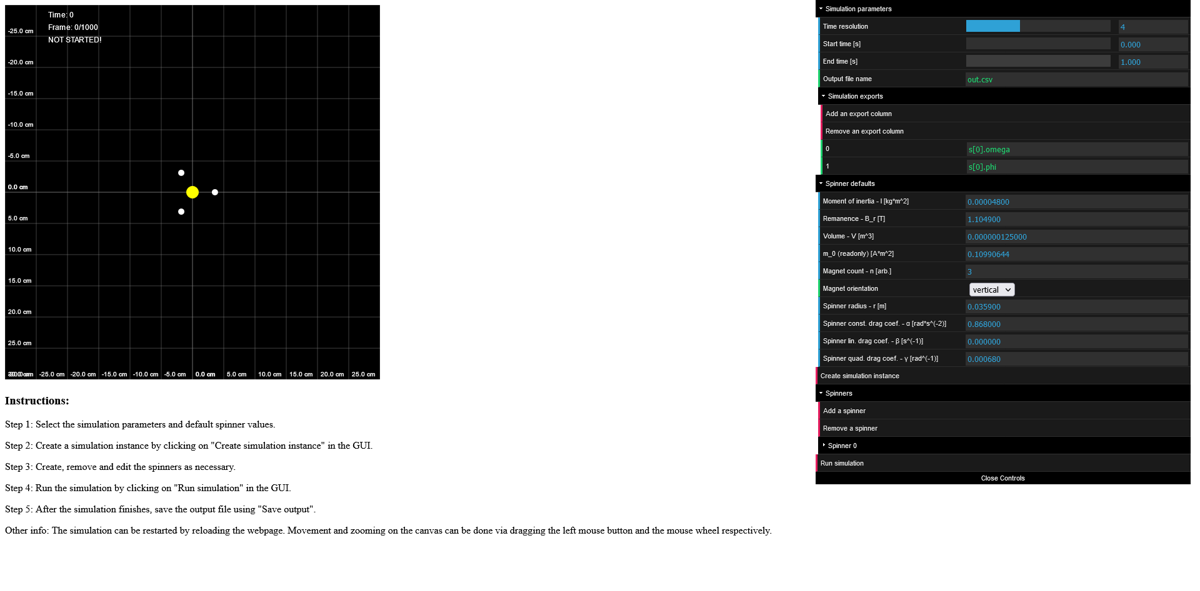
\includegraphics[width=0.9\textwidth]{screenshot_web_interface.png}
    \caption{Ukázka webového rozhraní}
    \label{fig:web_interface}
\end{figure}
\chapter{Potvrzení simulace}
\label{chap:sim_confirmation}

Po navržení a implementaci simulace je dalším krokem sledování její přesnosti a porovnání s reálnými experimenty. První způsob porovnání již byl zmíněn v \autoref{chap:drag}, kde jsme porovnávali simulované a reálné dopady tření na spinner a to bez externího magnetického pole (viz \autoref{fig:drag_fit}, \autoref{fig:drag_fit_wlin}) i v externím magnetickém poli (viz \autoref{fig:drag_fit_mag}, \autoref{fig:drag_fit_mag_wlin}). Všechna tato měření byla prozatím velmi podobná našim simulovaným hodnotám, avšak použit byl pouze jeden spinner. Další experimenty se tedy zaměří na další okrajové případy a použití více spinnerů.

\section{Vysokorychlostní videozáznam}

Nevýhodou minulého měření pomocí magnetického čidla Vernier je, že jsme nebyli schopni přesně určit okamžitou pozici, či rychlost. Toto nebyl tak velký problém, jelikož náš celkový záznam byl velmi dlouhý a nezajímaly nás mikroskopická chování spinneru, ale spíše makroskopický dopad tření na jeho schování. Nyní však budeme sledovat mikroskopické chování a to trackováním vyznačeného bodu na spinneru natočeného vysokorychlostní kamerou. K trackování použijeme volně dostupný software zvaný \texttt{Tracker} \cite{Tracker}. Snímkovou frekvenci jsme nastavili v jednom experimnetu na 60 snímků za sekundu, ve zbylých experimentech na 1000 snímků za sekundu.

\subsection{Aparatura}

%% literatura
\begin{thebibliography}{99}
    \bibitem{magnetic_force} YUNG, Kar W.; LANDECKER, Peter B. a VILLANI, Daniel D. An Analytic Solution for the Force Between Two Magnetic Dipoles. [Online]. \textit{Magnetic and Electrical Separation.} 1998, roč. 9, č. 1, s. 39-52. ISSN 1055-6915. Dostupné z: \url{https://doi.org/10.1155/1998/79537}. [cit. 2023-12-16].
    \bibitem{magnetic_torque} CULLITY, B. D. a GRAHAM, C. D. \textit{Introduction to magnetic materials.} Second edition. Hoboken: IEEE Press, [2009]. ISBN 978-0-471-47741-9.
    \bibitem{torque_def} SERWAY, Raymond A. a JEWETT, John W. Jr. \textit{Physics for scientists and engineers.} 6th ed. Belmont: Thomson-Brooks/Cole, 2004. ISBN 0-534-40842-7.
    % https://www.physicsforums.com/threads/modeling-a-permanent-magnetic-as-a-dipole.594949/#google_vignette
    % https://hal.science/hal-02905104/document
    \bibitem{magnet_dipole_approx} YE, Jianhe; ZHAN, Pengfei; ZENG, Jincheng; KUANG, Honglin; DENG, Yongfang et al. Concise magnetic force model for Halbach-type magnet arrays and its application in permanent magnetic guideway optimization. [Online.] \textit{Journal of Magnetism and Magnetic Materials.} 2023, roč. 587. ISSN 03048853. Dostupné z: \url{https://doi.org/10.1016/j.jmmm.2023.171301}. [cit. 2023-12-16].
    \bibitem{shorthand_error_notation} NATIONAL INSTITUTE OF STANDARDS AND TECHNOLOGY. \textit{Standard Uncertainty and Relative Standard Uncertainty} [online]. [cit. 2023-12-16]. Dostupné z: \url{https://physics.nist.gov/cgi-bin/cuu/Info/Constants/definitions.html}
    \bibitem{shorthand_error_notation_stack_exchange} Jasper. \textit{Shorthand error notation (with brackets) accros decimal point [duplicate]} [online]. [cit. 2023-12-16]. Dostupné z: \url{https://physics.stackexchange.com/questions/445141/shorthand-error-notation-with-brackets-accros-decimal-point}
    \bibitem{tmf_tasks} \textit{Turnaj mladých fyziků} [online]. [cit. 2023-12-16]. Dostupné z: \url{https://tmf.fzu.cz/tasks.php?y}
    \bibitem{magnet_grades} \textit{Neodymium Magnet Grades} [online]. [cit. 2023-12-16]. Dostupné z: \url{https://totalelement.com/blogs/about-neodymium-magnets/neodymium-rare-earth-magnet-grades}
    \bibitem{physical_pendulum} REICHL, Jaroslav a Martin VŠETIČKA. \textit{Fyzické kyvadlo} [online]. [cit. 2023-12-16]. Dostupné z: \url{http://fyzika.jreichl.com/main.article/view/206-fyzicke-kyvadlo}


    \bibitem{python} VAN ROSSUM, Guido, Drake VAN ROSSUM a L. FRED. \textit{Python 3 Reference Manual.} Scotts Valley, CA: CreateSpace, 2009. ISBN 1441412697.
    \bibitem{scipy} VIRTANEN, Pauli. SciPy 1.0: Fundamental Algorithms for Scientific Computing in Python. \textit{Nature Methods}. 2020(17), 261-272.
    \bibitem{numpy} HARRIS, Charles R. Array programming with NumPy. \textit{Nature.} 2020(585), 357–362.
    \bibitem{matplotlib} HUNTER, John D. Matplotlib: A 2D graphics environment. \textit{Computing in science \& engineering}. 2007, 9(3), 90-95.
    \bibitem{pymath} VAN ROSSUM, Guido. \textit{The Python Library Reference, release 3.8.2.} Python Software Foundation, 2020.
    \bibitem{phyphox} STAACKS, S; HÜTZ, S; HEINKE, H a STAMPFER, C. Advanced tools for smartphone-based experiments: phyphox. Online. \textit{Physics Education}. 2018, roč. 53, č. 4. ISSN 0031-9120. Dostupné z: \url{https://doi.org/10.1088/1361-6552/aac05e}. [cit. 2023-12-17].
    \bibitem{csv} SHAFRANOVICH, Yakov. Common format and MIME type for comma-separated values (CSV) files. \textit{RFC 4180, October}. 2005.

    \bibitem{spinner_mom_inert_external} ALLAIN, Rhett. Let’s Explore the Physics of Rotational Motion With a Fidget Spinner. \textit{WIRED} [online]. 2017, \textbf{2017}, 1-1 [cit. 2023-12-19]. Dostupné z: \url{https://www.wired.com/2017/05/physics-of-a-fidget-spinner/}

    \bibitem{sim_methods} STEWART, Robinson. \textit{Simulation – The practice of model development and use.} 1. John Wiley, 2004. ISBN 978-0-470-84772-5.
    \bibitem{RK_def} PRESS, William H. \textit{Numerical recipes: the art of scientific computing.} 3rd ed. Cambridge: Cambridge University Press, 2007. ISBN 978-0-521-88068-8.
    \bibitem{Butcher_tab_def} ISERLES, A. \textit{A first course in the numerical analysis of differential equations.} Cambridge: Cambridge University Press, 1996. ISBN 978-0-521-55655-2.
    \bibitem{RK_methods_list} PCC, Ben. WIKIMEDIA FOUNDATION. \textit{List of Runge–Kutta methods} [online]. 2007, 2023-12-20 [cit. 2023-12-22]. Dostupné z: \url{https://en.wikipedia.org/wiki/Runge–Kutta_methods}

    \bibitem{JS} FLANAGAN. \textit{JavaScript: the definitive guide.} O'Reilly Media, 2006.
    \bibitem{JSON} PEZOA, Felipe; REUTTER, Juan L.; SUAREZ, Fernando; UGARTE, Martín a VRGOČ, Domagoj. Foundations of JSON Schema. Online. In: \textit{Proceedings of the 25th International Conference on World Wide Web.} Republic and Canton of Geneva, Switzerland: International World Wide Web Conferences Steering Committee, 2016, s. 263-273. ISBN 9781450341431. Dostupné z: \url{https://doi.org/10.1145/2872427.2883029}. [cit. 2023-12-22].
    \bibitem{NodeJS} PEREIRA, Caio Ribeiro a PEREIRA, Caio Ribeiro. Introduction to Node.js. Online. In: \textit{Building APIs with Node.js}. Berkeley, CA: Apress, 2016, s. 1-3. ISBN 978-1-4842-2441-0. Dostupné z: \url{https://doi.org/10.1007/978-1-4842-2442-7_1}. [cit. 2023-12-22].
    \bibitem{IEEE-754}GANSSLE, Jack. IEEE 754 Floating Point Numbers. Online. In: \textit{The Firmware Handbook.} Elsevier, 2004, s. 203-205. ISBN 9780750676069. Dostupné z: \url{https://doi.org/10.1016/B978-075067606-9/50019-9}. [cit. 2023-12-22].
    \bibitem{JS_deconstruction} MOZILLA. Mozilla Developer Network. \textit{Destructuring assignment} [online]. [cit. 2023-12-27]. Dostupné z: \url{https://developer.mozilla.org/en-US/docs/Web/JavaScript/Reference/Operators/Destructuring_assignment}

    \bibitem{Tracker} \textit{Tracker - Video Analysis and Modeling Tool} [online]. 2008 [cit. 2024-01-03]. Dostupné z: \url{https://physlets.org/tracker/}
\end{thebibliography}

%% obrázky
\listoffigures

%% tabulky
\listoftables

%% snippety
\lstlistoflistings


\chapter*{Přílohy}
\begin{enumerate}[topsep=0pt, partopsep=0pt]
    \setlength{\itemsep}{0pt}%
    \setlength{\parskip}{0pt}%
    \item \label{attachment_1} Videozáznam interakce nehybného a pomalého spinneru \dotfill \textbf{VID1}
    \item \label{attachment_2} Videozáznam interakce nehybného a rychláho spinneru \dotfill \textbf{VID2}
    \item \label{attachment_3} Videozáznam interakce 3 spinnerů \dotfill \textbf{VID3}
\end{enumerate}
\end{document}